\documentclass[11pt,a4paper]{article}

% Basic packages
\usepackage[fontset=fandol]{ctex}
\usepackage{amsmath, amssymb}
\usepackage{graphicx}
\usepackage[margin=2.15cm]{geometry}
\usepackage[most]{tcolorbox}
\usepackage{etoolbox}
\usepackage{listings}
\usepackage{hyperref}
\usepackage{booktabs}
\usepackage{subcaption}
\usepackage{float}
\usepackage{tikz}
\IfFileExists{pgfplots.sty}{
    \usepackage{pgfplots}
    \pgfplotsset{compat=1.18}
}{}

% Highlight box palette: low-saturation and print-friendly.
% Visual weight is ordered by teaching role, so a page mixing several boxes still
% reads important > warning > knowledge > dialogue instead of competing for attention.
% Title text is white on every title bar; contrast stays within WCAG AA (4.5:1--6.0:1).
\definecolor{kbBack}{HTML}{F2F6FA}\definecolor{kbFrame}{HTML}{9DB4CC}\definecolor{kbTitle}{HTML}{52708F}
\definecolor{ibBack}{HTML}{FBF5E7}\definecolor{ibFrame}{HTML}{C9A961}\definecolor{ibTitle}{HTML}{7D5F1E}
\definecolor{wbBack}{HTML}{FCF2F0}\definecolor{wbFrame}{HTML}{D6A096}\definecolor{wbTitle}{HTML}{9E4F43}
\definecolor{dbBack}{HTML}{F4F7F3}\definecolor{dbFrame}{HTML}{AEC2AC}\definecolor{dbTitle}{HTML}{5F7F64}

\tcbset{softbox/.style={
    enhanced, boxrule=0.8pt, arc=2pt, left=3mm, right=3mm, top=2mm, bottom=2mm,
    coltitle=white, fonttitle=\bfseries, toptitle=0.6mm, bottomtitle=0.6mm
}}

% Highlight boxes
\newtcolorbox{knowledgebox}[1]{
    softbox, colback=kbBack, colframe=kbFrame, colbacktitle=kbTitle, title=#1
}

\newtcolorbox{importantbox}[1]{
    softbox, colback=ibBack, colframe=ibFrame, colbacktitle=ibTitle, title=#1
}

\newtcolorbox{warningbox}[1]{
    softbox, colback=wbBack, colframe=wbFrame, colbacktitle=wbTitle, title=#1
}

\newtcolorbox{dialoguebox}[1]{
    softbox, breakable, colback=dbBack, colframe=dbFrame, colbacktitle=dbTitle, title=#1
}

% Listings
\lstset{
    language=Python,
    basicstyle=\ttfamily\small,
    keywordstyle=\color{blue},
    stringstyle=\color{red!60!black},
    commentstyle=\color{green!60!black},
    breaklines=true,
    frame=single,
    numbers=left,
    numberstyle=\tiny\color{gray},
    captionpos=b,
    extendedchars=false
}


\usepackage{tabularx}
\newcolumntype{L}[1]{>{\raggedright\arraybackslash}p{#1}}
\hypersetup{colorlinks=true,linkcolor=kbTitle,urlcolor=kbTitle,pdftitle={CMU L3 长上下文管理：中文课程讲义},pdfauthor={Based on Graham Neubig; Chinese notes prepared with Codex}}
\renewcommand{\baselinestretch}{1.13}
\setlength{\parskip}{.4em}
\setlength{\emergencystretch}{2em}
\setcounter{tocdepth}{1}
\captionsetup{font=small,labelfont=bf}
\lstset{basicstyle=\ttfamily\footnotesize,columns=fullflexible,keepspaces=true,xleftmargin=6mm,framexleftmargin=4mm}
\begin{document}
\special{pdf:minorversion 7}
\hypersetup{pageanchor=false}
\begin{titlepage}
\centering
\vspace*{.9cm}
{\Large CMU 11-768 · AI Agents\par}
\vspace{.6cm}
{\Huge\bfseries 长上下文 Agent 的上下文管理\par}
\vspace{.4cm}
{\Large 模型架构、缓存与压缩的协同\par}
\vspace{.5cm}
{\large L3 中文课程讲义\par}
\vspace{1cm}
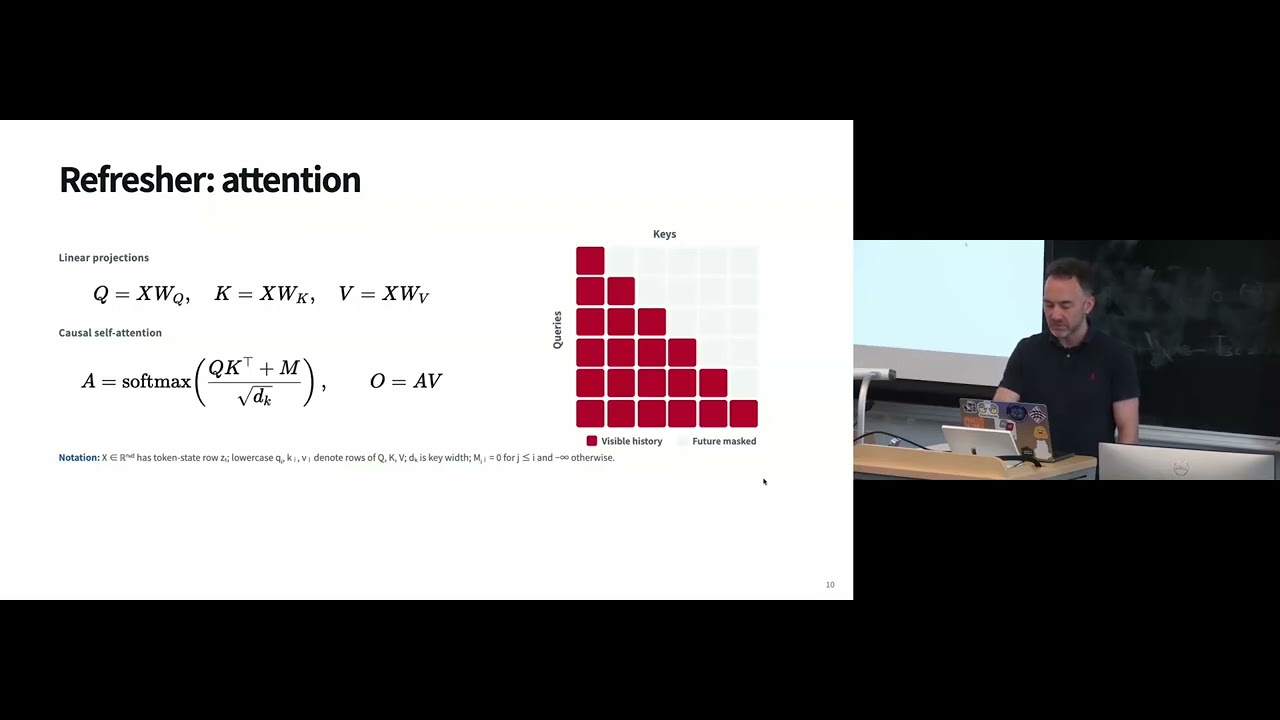
\includegraphics[width=\textwidth]{figures/原视频封面.jpg}\par
{\small 图：原视频封面\par}
\vfill
\begin{tcolorbox}[colback=kbBack,colframe=kbFrame,width=\textwidth]
\textbf{主讲 / 频道}：Graham Neubig\par
\textbf{课程}：Carnegie Mellon University，11-768 AI Agents，Fall 2026\par
\textbf{时长}：75 分 39 秒\par
\textbf{整理日期}：2026 年 10 月 2 日\par
\textbf{原视频}：\href{https://www.youtube.com/watch?v=AiwCCvFW1uE}{youtube.com/watch?v=AiwCCvFW1uE}
\end{tcolorbox}
\end{titlepage}
\pagenumbering{arabic}
\hypersetup{pageanchor=true}
\section*{本讲概览}
Agent 每完成一步，历史就会增加新的推理、工具调用和环境反馈。下一步既要利用这些信息，又要控制反复处理它们的计算与存储成本。本讲从历史增长出发，展开模型推理、长上下文架构与训练，再讨论前缀缓存和上下文压缩，最后把这些机制连接为完整系统。

本讲义依据带时间课程转录与官方课件整理，并结合原始论文核对机制。图示采用官方课件矢量裁图或注明的教学重绘；图注给出官方 PDF 页码，口述区间用于定位讲解。公式、代码与进一步归纳按其教学作用展开；模型实例与价格表保留课程时点，服务于机制比较。
\tableofcontents
\clearpage
\section{Agent 的历史为什么迅速变长}

\subsection{上下文既承载任务，也承载行动的后果}

普通的一次问答可以在回答后结束；Agent 往往需要持续行动。它读文件、解释结果、调用工具、遇到错误、修正方案，然后再次请求模型决定下一步。为了让下一次决策知道已经发生了什么，系统通常把此前的消息、工具调用和工具结果继续放进输入。因此，上下文管理首先是一个任务连续性问题：哪些证据和约束必须随任务一起保留下来？

本讲以长上下文语言模型的结构和服务系统为基础，再讨论 Agent 如何整理历史。讲者强调，这些机制并非只属于 Agent；Agent 的多轮执行使它们更容易成为实际瓶颈。

\subsection{线性增加的历史，如何造成二次增加的累计输入}

先看课件中的简化例子：固定前缀为 1K token，每轮新增约 5K token。五次模型调用的输入分别为 6K、11K、16K、21K、26K；最后一次输入只有 26K，五次累计输入却达到 80K。原因是旧历史在后续调用中被再次提交。

\begin{figure}[H]
\centering
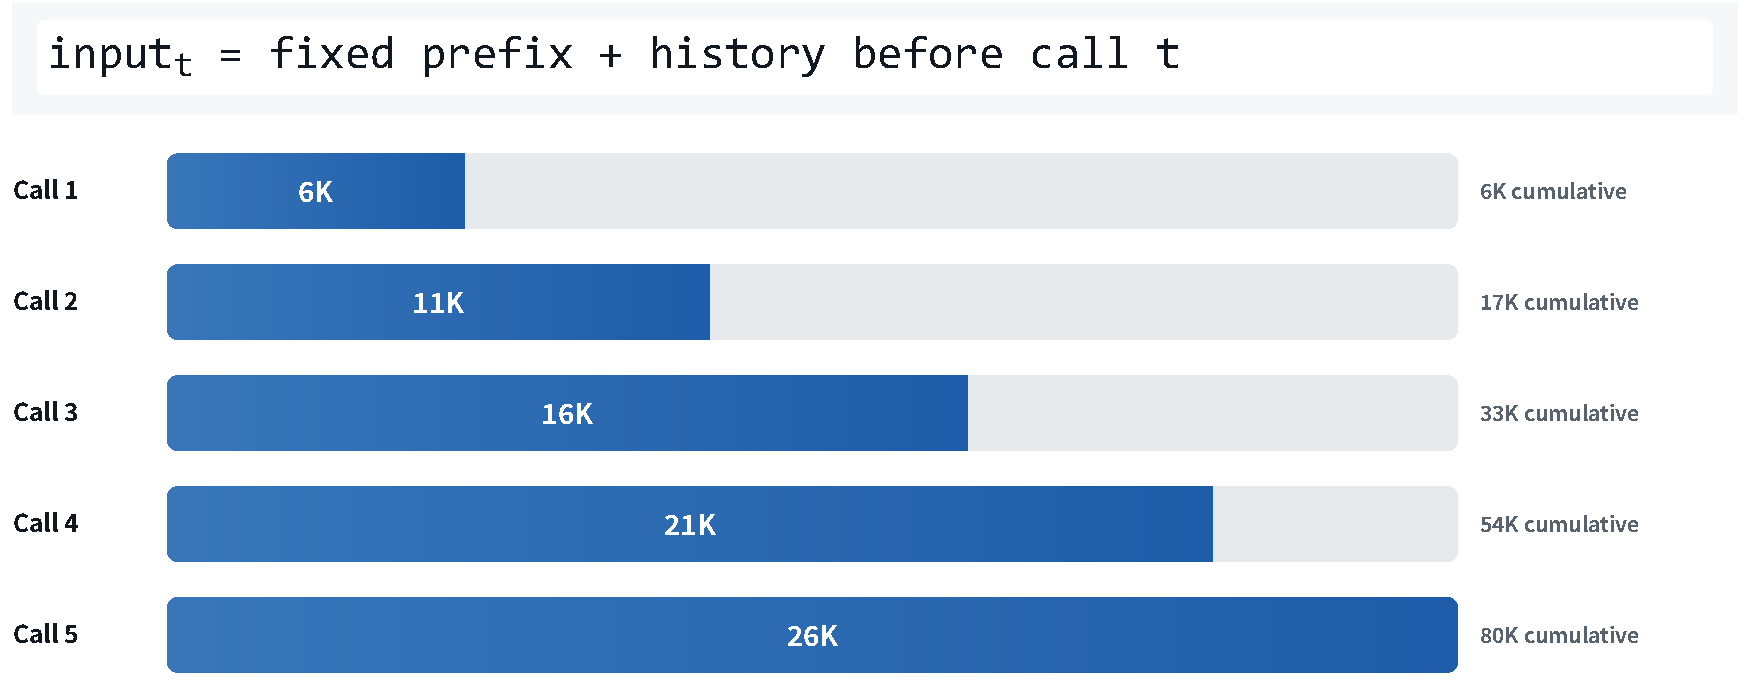
\includegraphics[width=\textwidth]{figures/历史增长与累计输入.pdf}
\caption{每次输入增长与累计输入增长是两个量。官方课件第 3 页。\newline{\footnotesize 对应口述 00:01:10--00:02:30。}}
\end{figure}

把这个例子推广：如果每次调用都提交完整历史，固定前缀被重复提交多次，而每轮新增内容还会在之后的调用中继续出现。累计输入长度是一个等差数列的和：
$$
L_t=p+tg,\qquad
C_T=\sum_{t=1}^{T}L_t=Tp+g\frac{T(T+1)}{2}.
$$
\begin{itemize}
\item $L_t$：第 $t$ 次调用的输入 token 数。
\item $p$：每次都保留的固定前缀长度，例如系统指令和工具说明。
\item $g$：简化假设下每轮新增的历史长度。
\item $t$：当前调用编号，从 1 开始。
\item $C_T$：前 $T$ 次调用累计提交的输入 token 数。
\item $T$：总调用次数。
\end{itemize}

实际每轮新增的长度并不相同。一条短工具结果和一整个源文件会产生不同增量，但这个例子揭示了共同机制：\textbf{历史的保留使一次新增内容参与多次后续决策。}

\begin{warningbox}{两种“二次增长”需要分别理解}
上述二次增长计算的是多次调用累计提交的输入长度。另一个二次复杂度来自单次全局注意力内部的 token 两两比较。这两件事出现在不同层面，不能把累计输入 token 数直接当成 GPU 运算量，也不能据此认定每次都必须重算全部历史。后文的 KV 缓存和前缀复用会改变重复前缀的计算与计费方式。
\end{warningbox}

\subsection{一份编码 Agent 记录中，谁占用了上下文}

讲者分析了 1,500 次 OpenHands 会话。这些会话主要是单个任务，并非连续多天工作的极长会话。课件报告的平均会话 token 数为 \textbf{77,922}。这个数字展示了该批数据的规模；它并不是所有 Agent 都应达到的长度。

\begin{figure}[H]
\centering
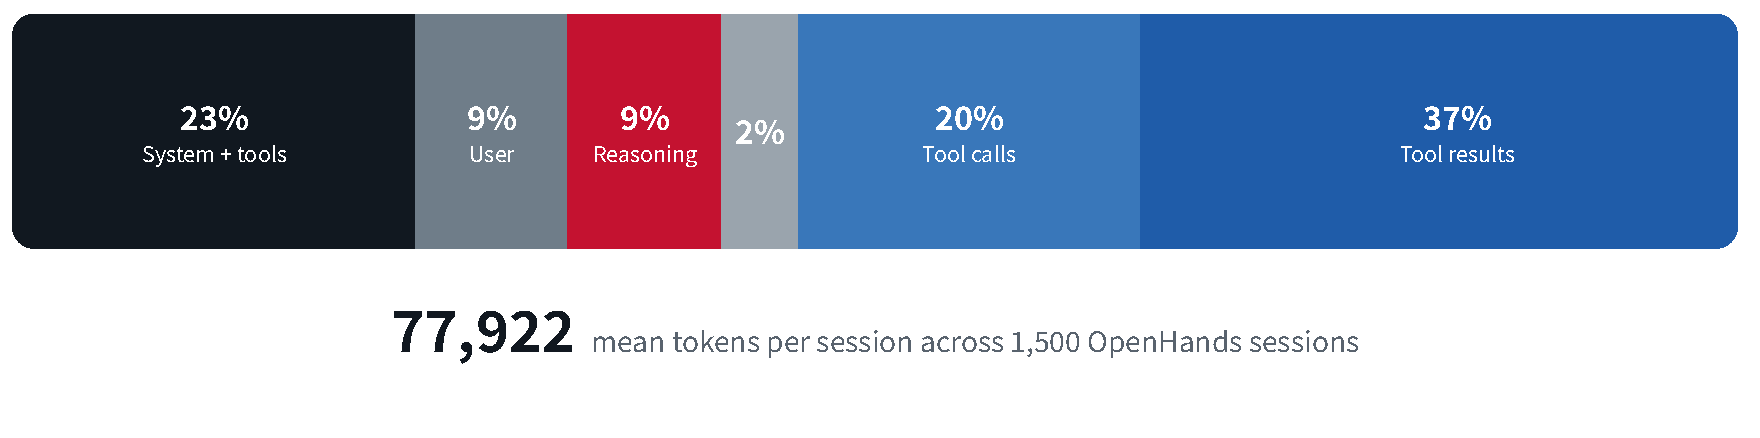
\includegraphics[width=\textwidth]{figures/OpenHands会话提示构成.pdf}
\caption{OpenHands 样本中的提示构成。官方课件第 4 页；图中 2\% 的类别由讲者口述补充为模型对用户的回复。\newline{\footnotesize 对应口述 00:02:30--00:05:05。}}
\end{figure}

各部分的作用如下：
\begin{itemize}
\item \textbf{23\%：系统指令与工具描述。} 固定规则和调用接口本身就是较大输入。
\item \textbf{9\%：用户消息。} 包括初始任务，以及执行中追加的约束和说明。
\item \textbf{9\%：推理轨迹。} 用于分析现状和决定后续行动的中间推理。
\item \textbf{2\%：模型直接回复用户的文字。} 这只是执行记录中较小的一部分。
\item \textbf{20\%：工具调用。} 例如读取代码、执行命令、写入修改；调用参数本身也会增长。
\item \textbf{37\%：工具结果。} 例如文件内容、命令输出和错误信息。
\end{itemize}

工具调用与工具结果合计占 57\%。对于编码 Agent，读一份文件或返回一段运行日志都可能带入大量文字；只观察聊天窗口里简短的最终回答，会低估执行历史的规模。讲者还指出，系统提示会随工具数量和行为规范而明显变化。固定前缀很大、工具返回内容很长、行动轮数很多，都会加剧上下文压力。

\begin{importantbox}{管理上下文，需要管理行动留下的证据}
Agent 的上下文并不等同于人与模型交谈的文字。系统规则、工具接口、调用参数和观测结果共同组成模型下一步决策的依据。整理历史时，应先确定每类内容承担什么作用，再决定它能否被缓存、筛选或压缩。
\end{importantbox}

\subsection{能力与效率：两个同时成立的要求}

长上下文面临两类挑战。第一类是\textbf{能力}：模型能否找到并利用当前任务需要的证据？架构、位置编码和训练数据决定模型获得什么能力；评价任务检验这些能力是否有效。第二类是\textbf{效率}：系统能否以可接受的成本和时延提供这种能力？注意力计算、KV 内存、缓存复用和上下文压缩共同影响服务效率。

这两类要求相互关联。一个能接收很长输入但难以找回早期约束的模型，会在 Agent 行动中产生错误；一个能正确利用历史但每次决策都等待很久的系统，也会限制交互和任务吞吐。后续内容围绕同一个问题展开：\textbf{怎样让任务所需的信息持续可用，同时控制使用它的代价？}

\subsection{本章小结}

Agent 每次行动都会产生新的历史；保留完整历史又使旧内容参与后续调用，累计输入会快速增长。OpenHands 的统计展示了系统规则和工具交互的体量。长上下文管理同时面对信息利用能力和服务效率，评价时需要分别观察这两方面。

\clearpage
\section{长上下文如何进入推理服务系统}

\subsection{从请求到响应：模型计算只是服务栈的一部分}

一份提示抵达服务端后，通常要经过排队、批处理和路由，然后执行模型计算，并逐步返回输出。多个请求共享计算设备，因此调度器既要安排任务，也要考虑每个请求留下的状态。课件将这套流程分成请求、调度器、Prefill、Decode、KV 缓存和响应。

\begin{figure}[H]
\centering
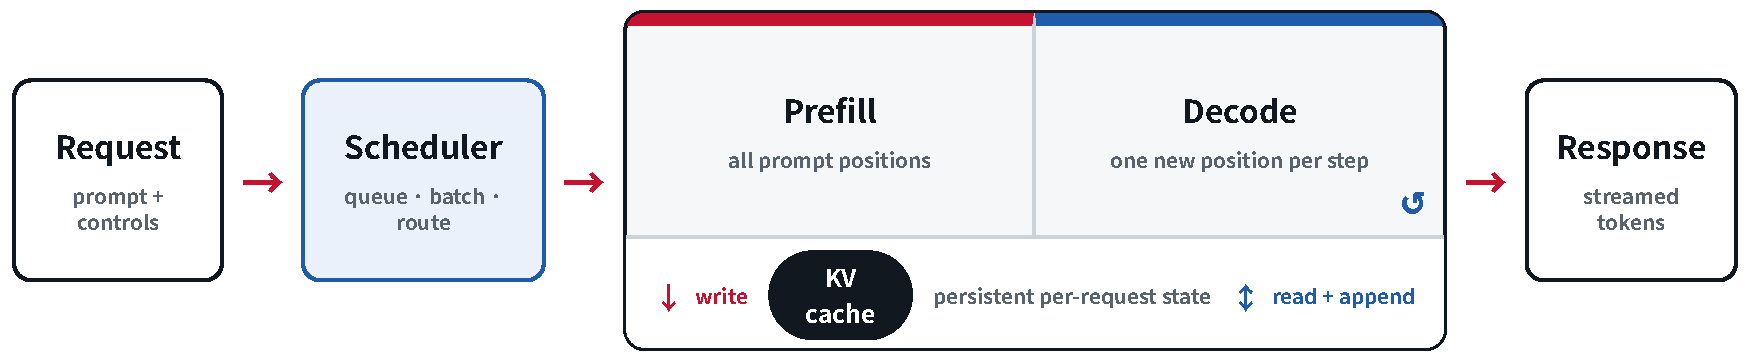
\includegraphics[width=\textwidth]{figures/推理服务栈与KV缓存.pdf}
\caption{推理服务栈中的调度、计算与持久状态。官方课件第 7 页。\newline{\footnotesize 对应口述 00:05:51--00:07:53。}}
\end{figure}

\subsection{Prefill 建立状态，Decode 读取并追加状态}

\textbf{Prefill（预填充）}处理已经给定的输入 token，为各层生成需要保存的 key 和 value。输入位置已知，因此可以一起组织计算。\textbf{Decode（解码）}按自回归顺序产生输出：根据现有历史状态预测新 token，再在后续步骤处理该 token 并将它的 KV 追加到缓存。输出尚未产生时，后面的生成位置无法像已知输入那样全部同时计算。

\begin{figure}[H]
\centering
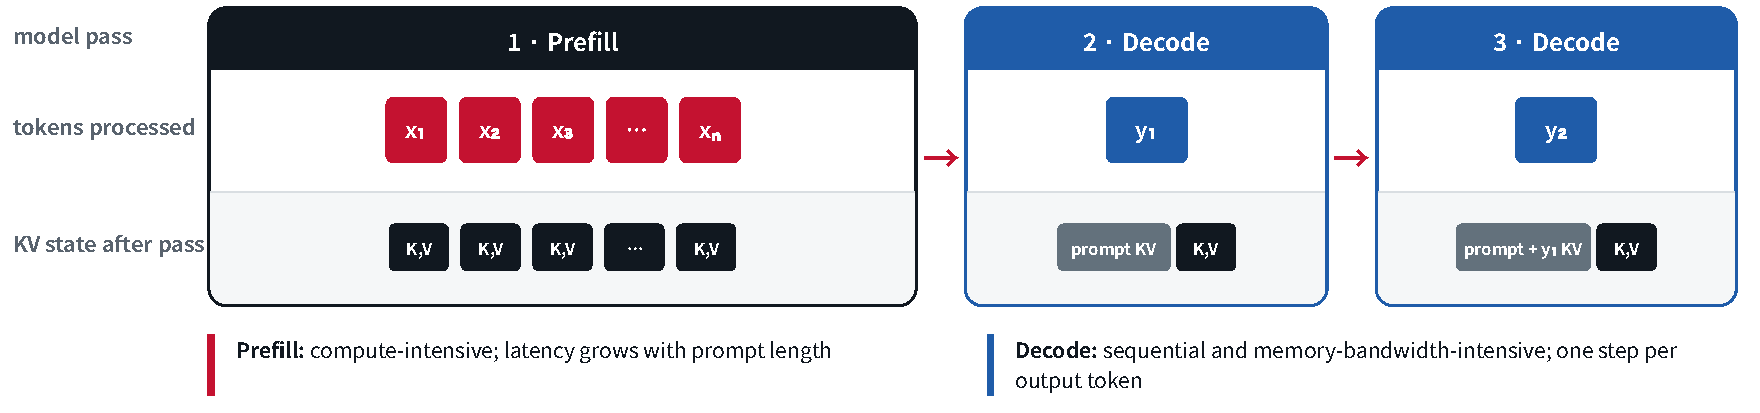
\includegraphics[width=\textwidth]{figures/Prefill与Decode状态演化.pdf}
\caption{预填充为输入建立 KV 状态，后续解码步骤复用并扩展状态。官方课件第 8 页。\newline{\footnotesize 对应口述 00:06:47--00:07:53。}}
\end{figure}

课件将 Prefill 概括为偏计算密集、时延随提示长度增加，将 Decode 概括为顺序执行且偏内存带宽密集。这是理解服务瓶颈的起点；实际瓶颈还取决于模型结构、批大小、硬件和缓存实现。

\begin{knowledgebox}{KV 缓存保存什么，又没有省掉什么}
缓存保存旧位置的 key/value，从而避免在每个解码步骤重新投影和处理整份历史。对于标准全局注意力，\textbf{新 query 仍要与历史 key 比较，并读取相应 value}。因此缓存能省去旧状态的重复构建，却没有消除新位置访问长历史的代价。跨请求的公共前缀复用，还需要服务系统能识别并保留相同前缀；后文会进一步讨论。
\end{knowledgebox}

\subsection{四类指标，对应四种观察角度}

等待开始输出的时间，与输出过程中继续等待的时间，需要分开测量。\textbf{TTFT}（Time to First Token）从请求到达开始计时，直到第一个输出 token 可见，可能包含排队和预填充。\textbf{TPOT}（Time per Output Token）关注后续 token 之间的平均间隔。

\begin{figure}[H]
\centering
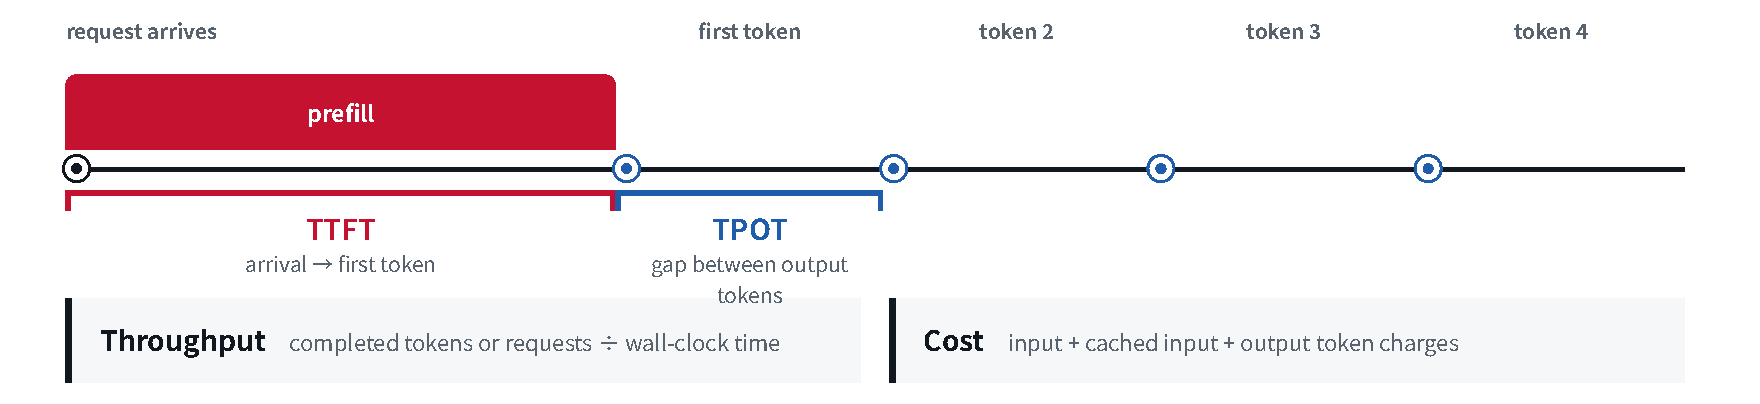
\includegraphics[width=\textwidth]{figures/首Token与逐Token时延.pdf}
\caption{首 token 时延、后续 token 间隔，以及系统级吞吐与费用。官方课件第 9 页。\newline{\footnotesize 对应口述 00:07:53--00:11:44。}}
\end{figure}

为了明确计时范围，设一次响应至少生成两个 token。可以用以下方式概括首 token 时延和平均输出间隔：
$$
\mathrm{TTFT}=\tau_1-\tau_a,\qquad
\mathrm{TPOT}=\frac{\tau_m-\tau_1}{m-1}.
$$
\begin{itemize}
\item $\mathrm{TTFT}$：从请求到达到首 token 的时间。
\item $\mathrm{TPOT}$：首 token 之后的平均 token 间隔。
\item $\tau_a$：请求到达时刻。
\item $\tau_1$：第一个输出 token 可见的时刻。
\item $\tau_m$：最后一个输出 token 可见的时刻。
\item $m$：此次响应的输出 token 总数，假设 $m\geq 2$。
\end{itemize}

\textbf{吞吐量}衡量一段真实时间内，整个系统完成了多少 token 或请求。\textbf{成本}衡量提供这些输出需要付出多少费用。课件展示了输入、缓存输入、输出 token 的收费划分；具体计价仍由所用服务决定。单个请求输出很快，不足以说明系统同时处理大量请求时的总吞吐高；系统吞吐高，也不足以说明每个交互请求都能很快开始响应。

讲者用两个 Agent 场景解释这些差别。人与编码 Agent 一起工作时，会反复等待下一步行动，首 token 时延和生成速度直接影响体验。让 Agent 在后台整夜处理任务时，用户可能更关注完成任务的总量和成本。因此，服务优化需要先明确工作负载的目标。

\begin{warningbox}{先读清楚“速度”的单位和计时范围}
token/秒与秒/token 方向相反。服务页面上的输出速率通常侧重解码阶段，不能直接代替包含预填充和排队的 TTFT。讲者展示服务商差异是为了说明服务系统会影响 Agent 体验；这些展示不是跨模型、跨时间都固定成立的排名。
\end{warningbox}

\subsection{标准注意力：每个位置如何选择历史信息}

一个输入位置先由隐藏表示投影出三类向量。query 表示当前要寻找的内容，key 表示可供匹配的内容，value 表示找到后要取出的信息。把多个 token 一起写成矩阵，就是：
$$
Q=XW_Q,\qquad K=XW_K,\qquad V=XW_V.
$$
\begin{itemize}
\item $X\in\mathbb{R}^{n\times d}$：输入 token 的隐藏状态矩阵，每行对应一个位置。
\item $n$：序列位置数。
\item $d$：隐藏状态宽度。
\item $Q\in\mathbb{R}^{n\times d_k}$：query 矩阵。
\item $K\in\mathbb{R}^{n\times d_k}$：key 矩阵。
\item $V\in\mathbb{R}^{n\times d_v}$：value 矩阵。
\item $W_Q,W_K,W_V$：可学习的投影矩阵。
\item $d_k$：query/key 向量宽度。
\item $d_v$：value 向量宽度。
\end{itemize}

随后，query 与各个 key 比较，将分数经 softmax 转为非负且和为 1 的权重，再用这些权重汇总 value。自回归模型通过因果掩码阻止一个位置读取未来 token：
$$
A=\operatorname{softmax}\!\left(\frac{QK^{\mathsf T}}{\sqrt{d_k}}+M\right),\qquad O=AV,
\qquad
M_{ij}=\begin{cases}0,&j\leq i,\\-\infty,&j>i.\end{cases}
$$
\begin{itemize}
\item $A\in\mathbb{R}^{n\times n}$：各 query 对各 key 的注意力权重矩阵；softmax 按行计算。
\item $Q,K,V$：上式定义的 query、key 和 value 矩阵。
\item $K^{\mathsf T}$：key 矩阵的转置。
\item $d_k$：key 宽度；平方根缩放用于控制点积分数的尺度。
\item $M$：因果掩码矩阵。
\item $i,j$：分别表示 query 位置与 key 位置。
\item $O\in\mathbb{R}^{n\times d_v}$：汇总后的注意力输出。
\item $-\infty$：被屏蔽位置的分数；经 softmax 后对应权重为 0。
\end{itemize}

以上写出一个注意力头的核心机制，省略多头拼接等外层结构。整段序列中，一个位置可比较此前所有位置，因此全局注意力的成对比较数量随序列长度二次增加。若只看一个已缓存历史上的新位置，它需要进行的是对历史长度呈线性增长的比较。

\subsection{能接收很长输入，能否有效利用也要检验}

课件展示了经典的 needle-in-a-haystack（大海捞针）实验：在很长的文章集合中插入一条可识别的事实，再向模型询问该事实。控制文章总长度和事实所在位置，可以检验模型是否能从不同位置找回证据。

\begin{figure}[H]
\centering
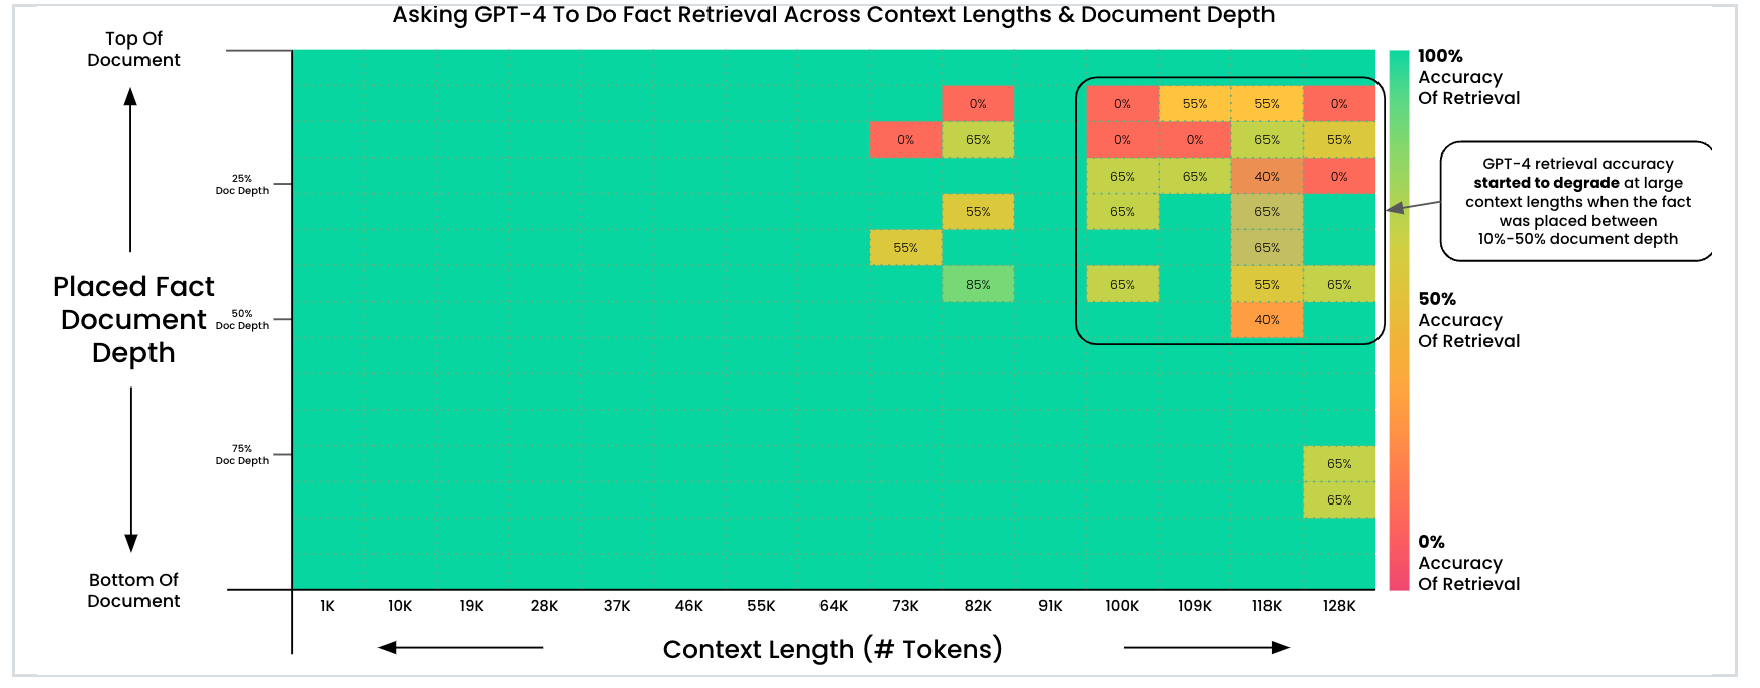
\includegraphics[width=\textwidth]{figures/长上下文针式检索评估.pdf}
\caption{检索准确率随上下文长度和事实插入位置变化的历史实验。官方课件第 11 页，引用 Kamradt（2023）的 GPT-4 评价。\newline{\footnotesize 对应口述 00:11:44--00:13:28。}}
\end{figure}

读图时，横轴是上下文长度，纵轴是被插入事实在文档中的相对位置，颜色表示检索准确率。较长输入中的一些位置出现黄、红区域，说明模型虽然接收了输入，仍可能没有可靠地利用其中的事实。讲者还提到 RULER 和 HELMET 等评价工作，作为进一步检查长上下文能力的途径。

这类单条事实检索并不覆盖 Agent 的全部需求。Agent 还可能要连接多个证据、跟踪状态变化，并遵守执行途中加入的限制。课堂讨论中，学生提到长会话会遗忘早期指令；讲者以忘记“不要删除”的约束为例说明：\textbf{历史信息丢失可能改变真实行动，而不只是降低问答得分。}

\begin{importantbox}{上下文窗口和有效上下文需要分别评价}
窗口大小描述系统允许输入多少内容。有效上下文能力描述模型能否在这些内容中找出、连接并使用任务需要的信息。长度限制、检索准确率、任务成功率和指令遵守，回答的是不同问题。
\end{importantbox}

\subsection{本章小结}

推理服务通过 Prefill 建立输入状态，再通过 Decode 逐步读取和追加状态。KV 缓存减少重复计算，却仍保留长历史访问的代价。TTFT、TPOT、吞吐和成本分别描述体验与资源使用；有效上下文则需要内容利用评价，不能由窗口长度替代。下面进入架构层，观察怎样减少访问历史的代价。

\clearpage
\section{架构路线：限制访问范围，或把历史写入状态}

\subsection{全局成对比较，为什么在极长序列上昂贵}

标准全局注意力允许当前位置直接读取此前任意位置。对长度为一百万 token 的序列，成对比较数量达到 $10^{12}$ 的数量级；因果注意力只保留下三角，但仍是同一二次数量级。每次比较还涉及向量计算，因此只增加硬件资源难以轻松承担极长序列。

讲者将许多改进概括为：给每个位置的计算设置上限，使整段序列的工作量随长度近似线性增加。不过，不同方法保留历史的方式不同。窗口方法保留附近 token 的直接访问；递归状态方法将更早的信息累积到固定大小的记忆；稀疏方法选择一部分远处位置；KV 压缩方法减少需要存取的历史表示。它们将在后续小节逐步展开。

\subsection{混合架构：让低成本机制与全局访问配合}

只使用很小的局部范围会限制直接获取远处信息的能力。课件展示的常见组合是：多个成本较低的局部或状态更新模块，与一个能够访问全局历史的模块交替出现。全局模块可以使用稠密注意力，也可以使用稀疏检索。

\begin{figure}[H]
\centering
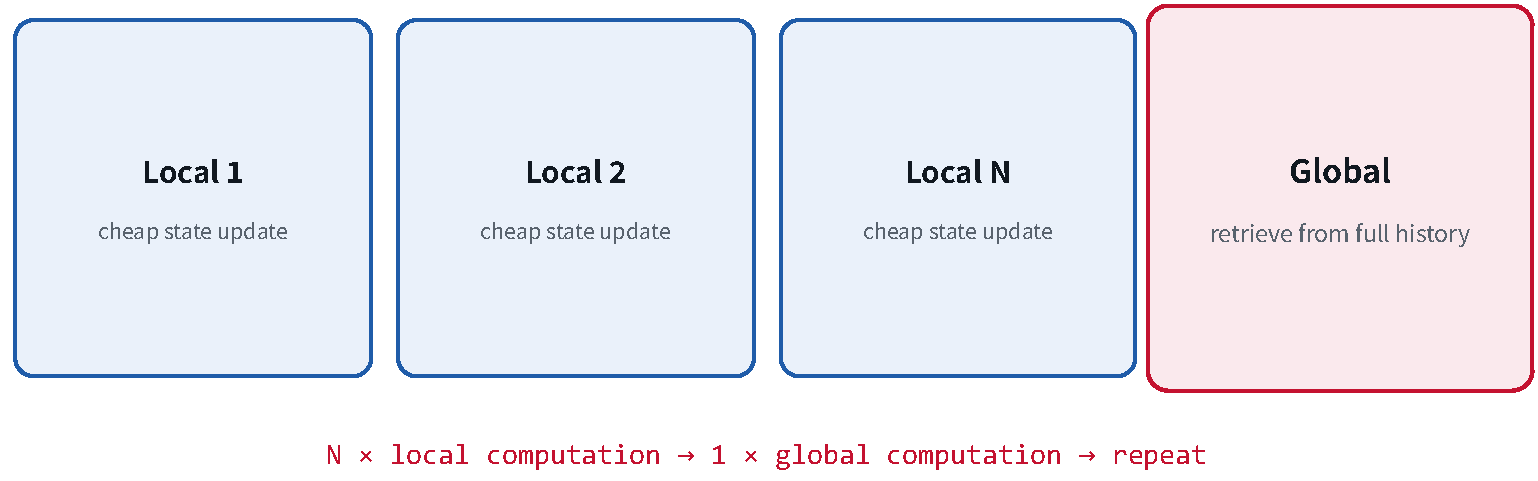
\includegraphics[width=0.93\textwidth]{figures/局部与全局混合结构.pdf}
\caption{多个低成本模块与全局访问模块组合的结构示意。官方课件第 15 页。\newline{\footnotesize 对应口述 00:16:43--00:18:50。}}
\end{figure}

\begin{figure}[H]
\centering
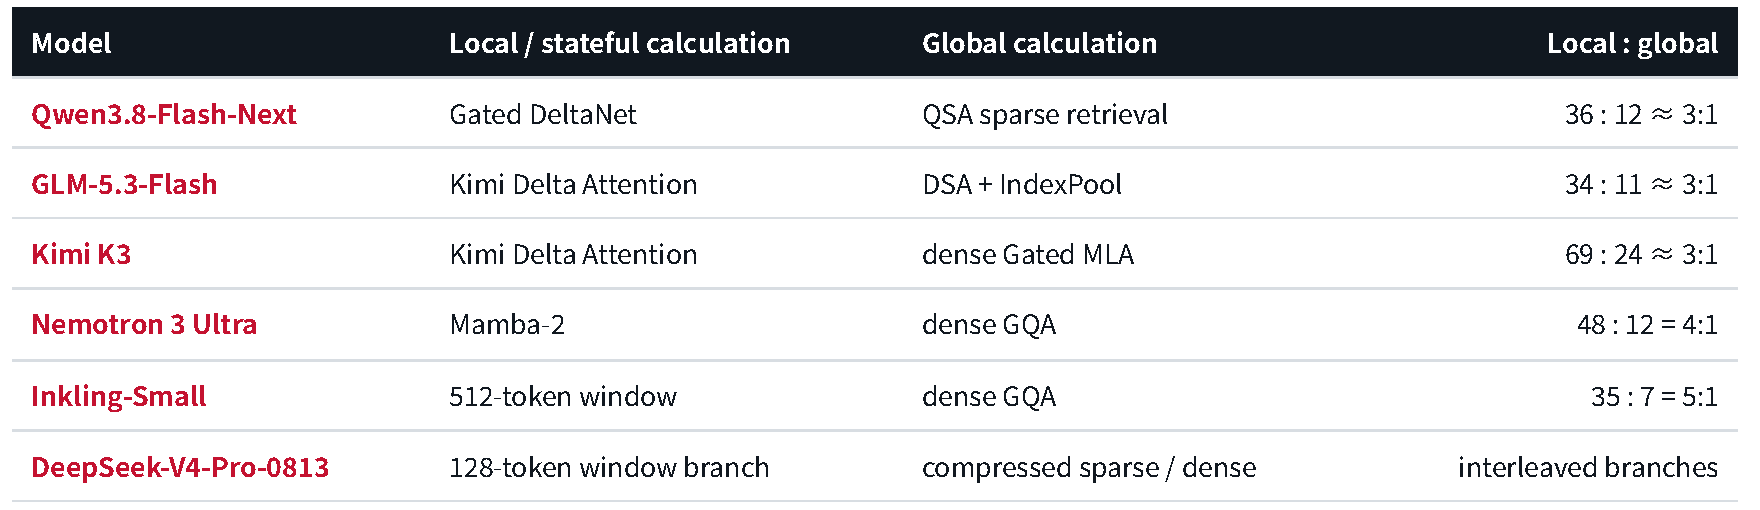
\includegraphics[width=\textwidth]{figures/课程列举的混合架构.pdf}
\caption{课程列举的六种混合架构及局部/全局模块配比。官方课件第 16 页。\newline{\footnotesize 对应口述 00:16:43--00:18:50。}}
\end{figure}

表中的配比展示局部/状态模块和全局模块的组成比例。它不是“每行动三次才读取一次历史”的 Agent 调用规则。课件中 Qwen、GLM 和 Kimi 的示例约为 3:1，Nemotron 约为 4:1，Inkling 约为 5:1；DeepSeek 示例则采用交错分支。它们选用的机制不同，但都试图减少昂贵全局计算的使用频率，同时保留远距离信息通路。

\begin{knowledgebox}{这里的“局部”也包括状态更新}
滑窗的局部性指只直接读取附近位置。递归状态更新的成本也受到控制，但状态可能承载整个过去的汇总。因此，课件将它们放在“Local / stateful calculation”这一栏。计算受限不意味着只能包含最近几个 token 的信息；关键要看远处信息是被直接读取，还是已经被写入状态。
\end{knowledgebox}

\subsection{滑动窗口：保留同一公式，改变可见位置}

滑动窗口注意力直接限制可访问的位置。每个 query 只能查看自己和之前固定范围内的 key，窗口之外及未来位置被屏蔽。其点积、softmax 和加权汇总机制保持不变，变化主要发生在掩码。

\begin{figure}[H]
\centering
\begin{subfigure}[t]{0.42\textwidth}
\centering
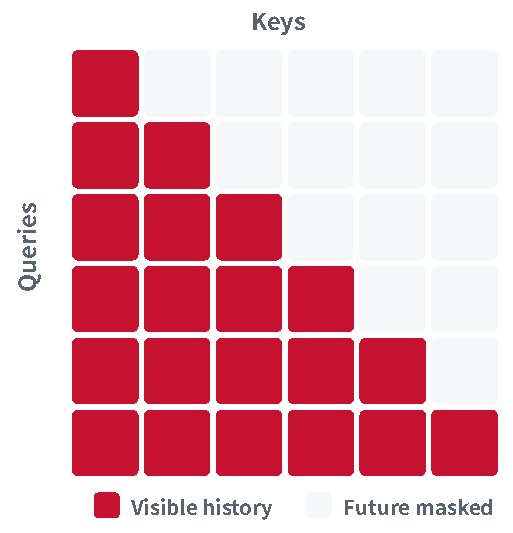
\includegraphics[height=4.5cm,keepaspectratio]{figures/标准因果注意力可见范围.pdf}
\caption{全局因果注意力}
\end{subfigure}\hfill
\begin{subfigure}[t]{0.42\textwidth}
\centering
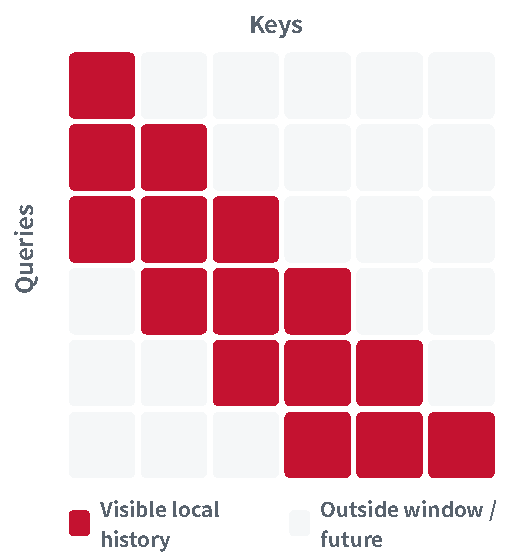
\includegraphics[height=4.5cm,keepaspectratio]{figures/滑窗因果注意力可见范围.pdf}
\caption{滑动窗口注意力}
\end{subfigure}
\caption{红色方格表示每个 query 能读取的 key。官方课件第 13、18 页。\newline{\footnotesize 对应口述 00:14:49--00:16:12，右图对应口述 00:18:50--00:20:02。}}
\end{figure}

用一个掩码明确窗口的边界；这里窗口宽度包含当前位置，所以每个 query 最多保留指定数量的因果位置：
$$
M_{ij}^{(w)}=\begin{cases}
0,&0\leq i-j<w,\\
-\infty,&\text{其他情况}.
\end{cases}
$$
\begin{itemize}
\item $M_{ij}^{(w)}$：query 位置 $i$ 对 key 位置 $j$ 的滑窗掩码值。
\item $i$：当前 query 位置。
\item $j$：被访问的 key 位置。
\item $w$：每个 query 保留的因果位置数，包含当前位置。
\item $0$：允许读取该位置，不改变原分数。
\item $-\infty$：禁止读取该位置，使其 softmax 权重为 0。
\end{itemize}

每个位置只比较至多一个窗口，整段序列的比较成本从 $O(n^2)$ 降到 $O(nw)$；其中 $n$ 是序列长度，$w$ 是窗口宽度。若窗口宽度保持固定，成本随序列长度线性增长。讲者用相邻块说明实现直觉，例如读取当前块和固定数量的前块；具体实现可以按 token 或按块组织可见范围。

单层窗口无法直接查找窗口之外的 token，但多层结构会扩大\textbf{有效感受野}。第一层把前一段的信息传给当前段，第二层又可利用前一段已经汇总过的信息，远处内容由中间表示逐层传来。这条间接通路解释了局部网络如何传播更长距离的信息，也解释了它为什么仍不能等同于一次直接检索所有历史：中间表示是否保留了所需细节仍是问题。

\begin{warningbox}{扩大感受野，不等于保证找回所有远处细节}
多层传播使远处信息有机会影响当前表示，但传递经过多个压缩和变换步骤。需要逐字读取旧代码、找回特定参数或遵守早期精细约束时，是否保留了那条具体信息，需要实际评价。窗口扩大或层数增加本身不能提供保证。
\end{warningbox}

\subsection{softmax 注意力为什么需要逐项比较}

在一个新位置上，全局注意力根据当前 query 对每个历史 key 的分数，重新构造一组权重。每项权重的分母依赖本次 query 对整个可见集合的评分，因此不同 query 可以聚焦不同历史位置。
$$
a_{ti}=\frac{\exp(q_t^{\mathsf T}k_i/\sqrt{d_k})}
{\sum_{j=1}^{t}\exp(q_t^{\mathsf T}k_j/\sqrt{d_k})},\qquad
o_t=\sum_{i=1}^{t}a_{ti}v_i.
$$
\begin{itemize}
\item $a_{ti}$：当前 query 对第 $i$ 个历史位置的归一化权重。
\item $q_t,k_i\in\mathbb{R}^{d_k}$：当前 query 与历史 key，使用列向量记法；$v_i\in\mathbb{R}^{d_v}$：历史 value。
\item $o_t\in\mathbb{R}^{d_v}$：当前位置的注意力输出。
\item $d_k,d_v$：query/key 与 value 的向量宽度。
\item $t$：当前位置，也是当前可见位置数；$i,j$：历史位置索引。
\item $\exp$：指数函数；分母把全部可见位置的正分数归一化。
\end{itemize}

这些权重非负、总和为 1，允许输出集中于最相关的少数 value。与此同时，生成每一组权重都需要访问相应的历史 key/value。保留完整 KV 缓存提供精细的 token 级读取能力，也使缓存体积随历史增长。

\subsection{线性注意力：利用结合律，先汇总再查询}

课程用一个简化推导解释线性注意力的核心思路：把归一化后的 softmax 权重换为双线性点积分数。这里发生了\textbf{模型计算规则的改变}，随后才使用代数结合律。这个教学式省去缩放和归一化，便于看清历史如何写入固定状态。

当前 query 可以先对每个 key 打分再加权 value，也可以先将全部 key/value 的外积加在一起，最后用 query 读取它：
$$
\widetilde{o}_t
=\sum_{i=1}^{t}(q_t^{\mathsf T}k_i)v_i
=\left(\sum_{i=1}^{t}k_i v_i^{\mathsf T}\right)^{\mathsf T}q_t
=S_t^{\mathsf T}q_t.
$$
\begin{itemize}\setlength{\itemsep}{2pt}\setlength{\parsep}{0pt}
\item $\widetilde{o}_t\in\mathbb{R}^{d_v}$：简化双线性机制的输出；加波浪号以区别于标准 softmax 输出。
\item $q_t,k_i$：当前位置 query 和历史 key，均为 $d_k$ 维列向量。
\item $v_i$：历史 value，为 $d_v$ 维列向量。
\item $k_i v_i^{\mathsf T}$：key/value 外积，得到 $d_k\times d_v$ 的矩阵。
\item $S_t\in\mathbb{R}^{d_k\times d_v}$：截至位置 $t$ 的外积累积状态；$\mathsf T$：矩阵转置。
\item $t$：当前序列位置；$i$：被累计的历史位置索引；$d_k,d_v$：key 与 value 的向量宽度。
\end{itemize}

这个变换的价值在于，状态只需要在旧状态上加一次当前写入，不必每次从头求和：
$$
S_0=0,\qquad S_t=S_{t-1}+k_t v_t^{\mathsf T},\qquad
\widetilde{o}_t=S_t^{\mathsf T}q_t.
$$
\begin{itemize}
\item $S_0$：初始全零状态；$S_{t-1}$：处理当前位置之前的状态；$S_t$：加入当前 key/value 后的状态。
\item $k_t,v_t$：当前位置的 key 和 value。
\item $q_t$：当前位置 query；$\widetilde{o}_t$：从更新后状态读取的双线性输出。
\item $t$：序列位置，从 1 开始更新；$\mathsf T$：矩阵转置；$0$：全零矩阵。
\end{itemize}

因此，在向量宽度固定的情况下，\textbf{每个 token 的状态更新与读取成本不随历史长度增加}，整段序列的递归计算随序列长度线性增加；保存的状态大小也不随 token 数增加。这里的“常数”是相对于序列长度而言，状态矩阵仍有维度，并不意味着计算或内存为零。这个递归更新形式也解释了线性注意力与循环神经网络之间的联系。

\begin{importantbox}{两种历史表示，提供两种读取能力}
标准 softmax 注意力保存逐 token 的 KV，再按当前 query 对每条历史重新评分。简化线性机制把历史关联累积到一个固定矩阵中，再以 query 读取这个矩阵。前者保留精细的显式历史访问，后者以有界状态换取随序列长度线性增长的计算。
\end{importantbox}

\subsection{得到效率之后，为什么还要改进记忆机制}

替换 softmax 后，点积分数可以为负，也不再保证相加为 1。输出失去原来对所有候选进行相对归一化选择的性质；历史关联写进同一矩阵，也可能互相干扰。若不断对同一 key 写入新 value，简单累加会把新旧关联叠在一起，缺少针对旧关联的清除或修正。

\begin{warningbox}{这条推导的两个边界}
双线性式与标准 softmax 注意力不是等价公式。实际线性注意力模型还可以加入特征映射、归一化和门控等机制，不能把上式视为全部线性模型的完整定义。另一个细节是：softmax 权重依赖 query，所以标准注意力作为 query 到输出的函数一般是非线性的；固定状态 $S_t$ 下的双线性读取，才是关于 query 的线性映射。
\end{warningbox}

后续 DeltaNet、Gated DeltaNet 和 Kimi Delta Attention 正是沿这条思路继续改进：保持递归状态的效率，并为记忆加入纠错或遗忘能力。理解简单累加留下的问题，才能看清这些更新规则各自增加了什么。

\subsection{本章小结}

降低长上下文代价有两条已经展开的路线：滑窗限制直接读取的位置，递归状态将历史关联写入固定记忆。混合模型为低成本模块保留全局访问通路。线性注意力的关键代数步骤是先改变评分机制，再通过结合律汇总历史；它带来效率，也引出归一化选择能力和状态干扰的问题。下一章将继续讨论如何纠正、遗忘和检索历史信息。



\clearpage
\section{高效记忆的进一步设计：定向纠错、稀疏读取与 KV 压缩}

固定大小的线性注意力状态解决了历史越长、逐次读取越贵的问题，但把全部历史写进一张矩阵也带来新的困难：重复写入同一个键时，旧值与新值可能叠加；不同键之间可能相互干扰；很久以前的信息可能持续影响当前预测。讲者接下来分别改进\textbf{写入规则、遗忘规则、读取范围和存储表示}。这四个方向处理的成本与失败方式各不相同。

\subsection{DeltaNet：先读取旧关联，再写入预测误差}

先把状态矩阵看作一个在线更新的键到值映射。新 token 提供一个键和值后，模型先询问现有记忆：“这个键目前会读出什么值？”随后用期望值减去读出的值，只把差额写回去。这样的写入能够纠正旧关联，避免每次都把完整的新值无条件累加到状态上。

沿用课件的矩阵方向，DeltaNet 的一次更新如下：
$$
\begin{aligned}
\widehat v_t &= S_{t-1}^{\top}k_t, & e_t &= v_t-\widehat v_t,\\
S_t &= S_{t-1}+\beta_t k_t e_t^{\top}, & o_t &= S_t^{\top}q_t.
\end{aligned}
$$
\begin{itemize}
  \item $t$：当前 token 的位置；$S_{t-1}\in\mathbb R^{d_k\times d_v}$、$S_t$：更新前后的记忆状态；$d_k$、$d_v$：键空间与值空间的维数。
  \item $k_t\in\mathbb R^{d_k}$、$v_t\in\mathbb R^{d_v}$：当前写入的键和值；$\widehat v_t$：旧状态对该键的预测；$e_t$：预测误差。
  \item $\beta_t\in[0,1]$：纠正强度，控制写回多少误差；$\top$：转置；$k_t e_t^{\top}$：一个秩一的外积更新。
  \item $q_t\in\mathbb R^{d_k}$：当前查询；$o_t\in\mathbb R^{d_v}$：更新后的读出结果。
\end{itemize}

这与学习率的直觉相近：纠正强度较小，就向新值靠近一部分；较大，则更积极地改写当前关联。不过这里更新的是推理过程中的动态状态，不能把它与离线训练模型参数的优化步骤混为一谈。

为了看清“纠正”究竟有多强，把更新后的状态再次用于读取\emph{同一个键}，可以得到下面的关系。这是由课件更新式直接推得的解释性补充：
$$
S_t^{\top}k_t
=\widehat v_t+\beta_t\lVert k_t\rVert_2^2\bigl(v_t-\widehat v_t\bigr).
$$
\begin{itemize}
  \item $S_t$：完成 Delta 更新的状态；$k_t$：再次查询的同一个键；$\top$：转置。
  \item $\widehat v_t$、$v_t$：更新前预测与期望写入值；$\beta_t$：纠正强度。
  \item $\lVert k_t\rVert_2^2$：键的平方欧氏范数，决定外积更新作用到这个键时的实际尺度。
\end{itemize}

若键的欧氏范数为 1，新的读出就在旧预测与新值之间插值。例如，旧预测是 2，目标值是 6，纠正强度取 $0.5$，新的读出就是 4；纠正强度取 1 时，这个键的读出成为 6。这是一个单值示例，实际值可以是向量。

\begin{warningbox}{“完全覆盖旧值”有条件}
单位范数键配合纠正强度 1，才会由上式直接得到同键的精确覆盖。未经归一化的键不能套用这一结论。更新也可能影响与当前键相关的其他查询：正交方向不会受到该秩一纠正的影响，非正交方向仍可能有干扰。因此，定向写入并不等于给每个历史 token 分配互不影响的独立存储格。
\end{warningbox}

\subsection{Gated DeltaNet 与 KDA：把“该改多少”与“该忘多少”分开}

DeltaNet 改进了写入方式，但过去的状态仍可能积累得过久。Gated DeltaNet 在纠正之前先衰减整个状态：先让旧记忆保留一定比例，再根据衰减后的预测写入误差。这样，\textbf{保留门负责遗忘，纠正门负责更新当前关联}。

其顺序与公式如下：
$$
\begin{aligned}
\widetilde S_{t-1}&=\alpha_t S_{t-1},\\
S_t&=\widetilde S_{t-1}
+\beta_t k_t\bigl(v_t-\widetilde S_{t-1}^{\top}k_t\bigr)^{\top}.
\end{aligned}
$$
\begin{itemize}
  \item $t$：当前位置；$S_{t-1}\in\mathbb R^{d_k\times d_v}$、$S_t$：更新前后的状态；$d_k$、$d_v$：键和值的维数。
  \item $\alpha_t\in[0,1]$：标量保留门；$\widetilde S_{t-1}$：经过衰减的旧状态。
  \item $k_t\in\mathbb R^{d_k}$、$v_t\in\mathbb R^{d_v}$：当前键和值；$\beta_t\in[0,1]$：误差纠正强度；$\top$：转置。
\end{itemize}

保留门越接近 0，遗忘越快；越接近 1，旧状态保留得越久。把保留门设为 1，就恢复为 DeltaNet。门可以随输入变化，因此“较近的信息更重要”能够成为可学习的状态更新行为，而不必完全依赖一个固定窗口。

Kimi Delta Attention（KDA）进一步给\textbf{每个键空间通道}一个独立的保留系数。某些特征可以缓慢衰减，某些特征可以快速更新，形成不同的记忆时间尺度。按照课件的状态方向，衰减矩阵从左侧作用于状态，也就是缩放状态的各行。

将逐通道衰减与定向纠正合起来，课件写成：
$$
\begin{aligned}
D_t&=\operatorname{Diag}(\boldsymbol\alpha_t),
&\widetilde S_{t-1}&=D_tS_{t-1},\\
S_t&=\bigl(I-\beta_t k_tk_t^{\top}\bigr)D_tS_{t-1}
+\beta_t k_tv_t^{\top}.
\end{aligned}
$$
\begin{itemize}
  \item $\boldsymbol\alpha_t\in[0,1]^{d_k}$：逐键通道的保留系数；$\operatorname{Diag}$：将向量构成对角矩阵；$D_t\in\mathbb R^{d_k\times d_k}$：衰减矩阵。
  \item $t$：当前位置；$S_{t-1}\in\mathbb R^{d_k\times d_v}$、$\widetilde S_{t-1}$、$S_t$：原状态、衰减状态和更新状态；$d_k$、$d_v$：键和值的维数。
  \item $I\in\mathbb R^{d_k\times d_k}$：单位矩阵；$k_t$、$v_t$：当前键和值；$\beta_t$：纠正强度；$\top$：转置。
\end{itemize}

若所有键通道采用相同的保留系数，KDA 的这一步就退化为标量门控的更新。这里“逐通道”不代表矩阵中每个单独的格子都有任意独立的遗忘值；课件采用的是\emph{键空间上的对角门}。

下面的教学重写用一段 NumPy 运算展示这个次序。假定键、值、查询与门值已经由模型产生，键非零；该片段演示单个状态的递推，不包含多头、分块训练或高性能内核。

\noindent\begin{minipage}{\textwidth}
\begin{lstlisting}[language=Python,caption={教学重写：逐通道衰减后，再按预测误差更新状态}]
import numpy as np

# S: (d_k, d_v), k and q: (d_k,), v: (d_v,)
# alpha: (d_k,), beta: scalar in [0, 1]
k = k / np.linalg.norm(k)
decayed = alpha[:, None] * S
prediction = decayed.T @ k
error = v - prediction
S = decayed + beta * np.outer(k, error)
output = S.T @ q
\end{lstlisting}
\end{minipage}

特别要注意，预测误差是相对于\emph{已经衰减的状态}计算的。若先用原状态预测，再把该误差写入衰减状态，就改变了上述更新规则。

\begin{importantbox}{递推记忆的三步演进}
线性注意力用固定矩阵累计关联；DeltaNet 在当前键方向上修正预测误差；Gated DeltaNet 与 KDA 再加入整体或逐通道遗忘。这些方法改善固定大小记忆的写入质量与时间尺度，但仍然要在有限状态中承载历史信息。讲者提到 Mamba 属于相近的递推建模方向，本课没有展开其更复杂的数学推导。
\end{importantbox}

\subsection{稀疏注意力：保留历史 token，但只读取选中的部分}

稀疏注意力采用另一种思路：继续保留可供查询的历史表示，只让当前查询读取其中一部分。\textbf{固定模式}按位置安排可见集合，例如局部窗口加少量全局位置；\textbf{内容相关模式}则根据当前查询选择历史位置。前者的连接结构可预先确定，后者更灵活，但需要额外的选择步骤。

\begin{figure}[H]
\centering
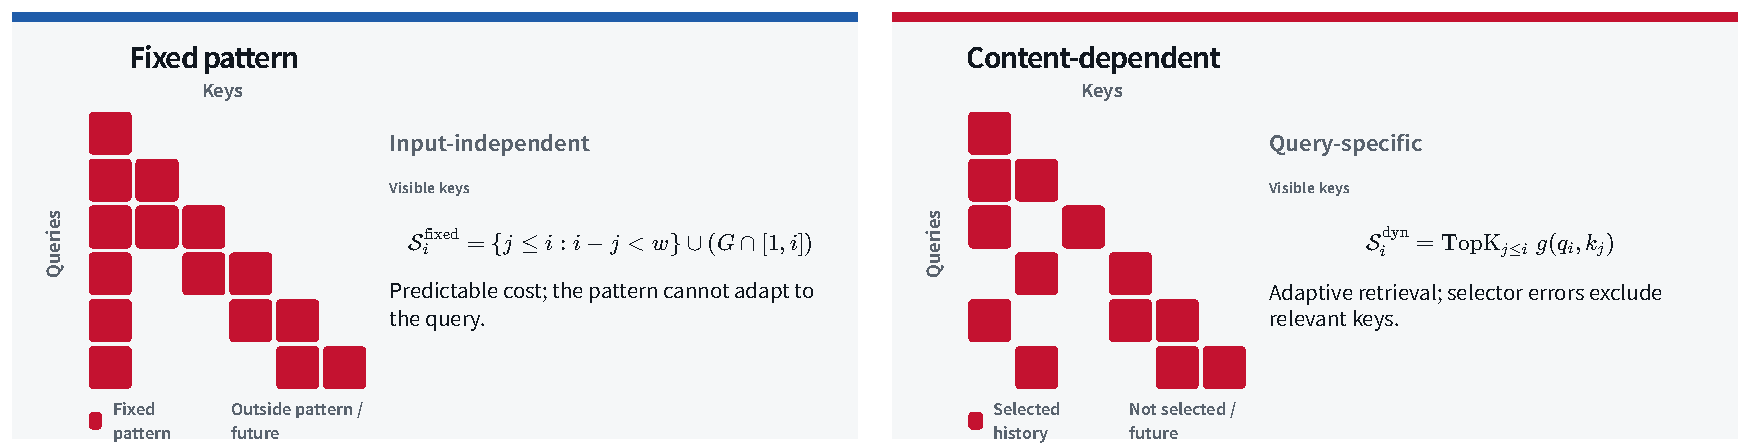
\includegraphics[width=\textwidth]{figures/稀疏注意力的固定与动态选择.pdf}
\caption{固定模式与内容相关选择。红色位置参与注意力，灰色位置被排除。来源：官方课件第 24 页的矢量裁图；对应口述 00:31:14--00:33:35。}
\end{figure}

课件用局部窗口加全局位置说明固定模式，并用学习到的选择器说明动态模式：
$$
\begin{aligned}
\mathcal S_i^{\mathrm{fixed}}
&=\{j\le i:i-j<w\}\cup\bigl(G\cap[1,i]\bigr),\\
\mathcal S_i^{\mathrm{dyn}}
&=\operatorname{TopK}_{j\le i}\,g(q_i,k_j).
\end{aligned}
$$
\begin{itemize}
  \item $i$：当前查询位置；$j$：候选历史位置，$j\le i$ 保持因果约束；$\mathcal S_i^{\mathrm{fixed}}$、$\mathcal S_i^{\mathrm{dyn}}$：最终可读取的位置集合。
  \item $w$：局部窗口大小；$G$：固定的全局位置集合；$[1,i]$：截至当前的合法位置范围；$\cup$、$\cap$：并集与交集。
  \item $q_i$、$k_j$：查询与候选键；$g$：较便宜的相关性选择函数；$\operatorname{TopK}$：选取评分最高的 $K$ 个候选，$K$ 是保留数量。
\end{itemize}

动态选择可以先将查询与键投影到较小的维度，计算便宜的评分，再只对选中的位置计算完整注意力。讲者把它概括为“先选、再算”的两次处理。在课堂问答中，他没有确认所有实现都采用余弦相似度，因此这里用一般的选择函数保留该实现差异。

选好集合后，模型在\emph{保留集合内部}重新归一化注意力，而不是继续沿用原来对全部历史归一化的权重：
$$
A_{ij}
=\frac{\exp(q_i^{\top}k_j/\sqrt{d_k})}
{\displaystyle\sum_{r\in\mathcal S_i}\exp(q_i^{\top}k_r/\sqrt{d_k})},
\qquad
o_i=\sum_{j\in\mathcal S_i}A_{ij}v_j,
\qquad j\in\mathcal S_i.
$$
\begin{itemize}
  \item $i$：查询位置；$j$、$r$：被保留的候选位置；$\mathcal S_i$：固定或动态得到的可读集合。
  \item $q_i$、$k_j$、$k_r$：查询与键；$d_k$：键维数；$\top$：转置；$\exp$：指数函数。
  \item $A_{ij}$：集合内部归一化后的权重；$v_j$：候选值；$o_i$：最终输出。
\end{itemize}

\begin{warningbox}{稀疏化的两类代价}
固定模式可能从结构上看不到某个远处证据；动态模式可能因为选择器评分错误而漏掉它。一旦相关位置未进入集合，后面的完整注意力也无法补读该位置。计算复杂度还要连同选择器一起计算：保留数量固定可降低完整注意力的工作量，但若选择器仍扫描全部历史，其代价不会凭空消失。固定比例的稀疏连接也可能只是降低二次成本的系数，并未改变其随长度增长的阶数。
\end{warningbox}

\subsection{GQA、MQA 与 MLA：减少每个历史 token 的缓存表示}

稀疏注意力主要减少“读取哪些位置”的工作；KV 压缩则减少“每个位置需要存多少东西”。标准多头注意力（MHA）为各个头缓存各自的键和值。分组查询注意力（GQA）让多组查询头共享更少的 KV 头；多查询注意力（MQA）是仅保留一组 KV 的极端情形。查询头仍可有不同的查询向量。

\begin{figure}[H]
\centering
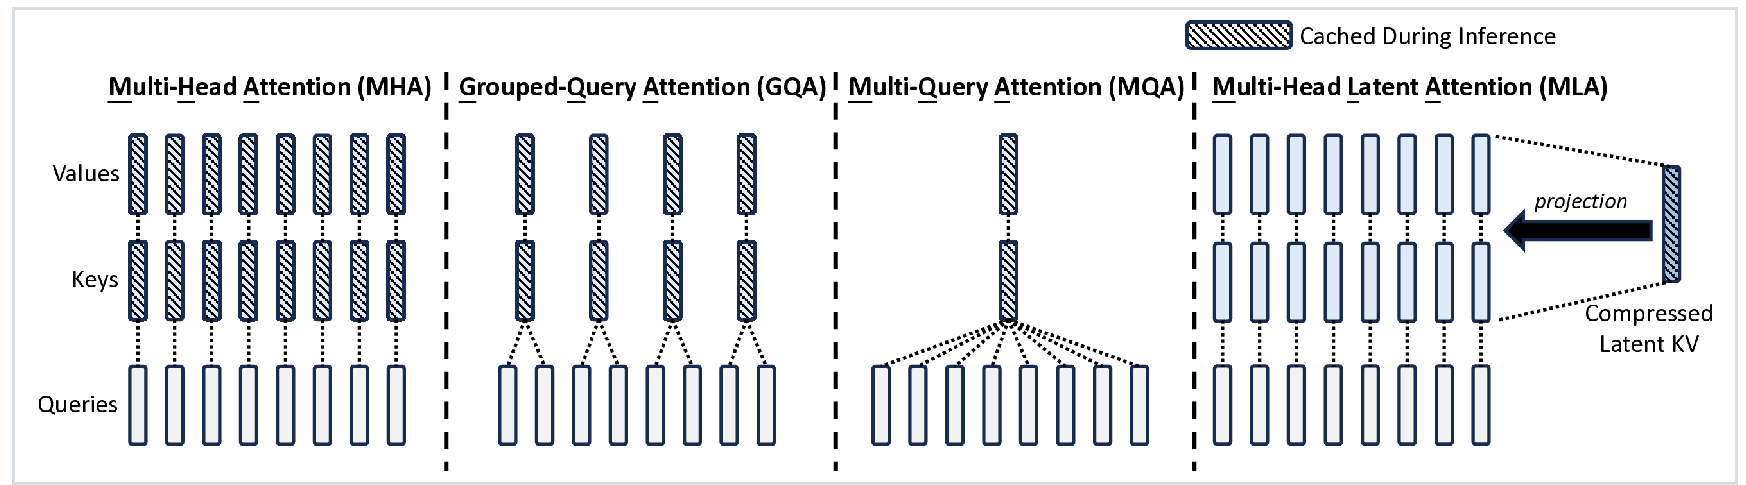
\includegraphics[width=\textwidth]{figures/MHA_GQA_MQA_MLA的缓存结构.pdf}
\caption{MHA、GQA、MQA 与 MLA 的缓存结构。斜线标记推理时需要缓存的部分。来源：官方课件第 25 页的矢量裁图；对应口述 00:33:35--00:35:57。}
\end{figure}

在相同键值维度、精度与层数下，KV 头数下降，缓存大小就按头数比例下降。用一个简化估计把这个关系写清楚：
$$
\mathrm{KV\ bytes}
\approx 2n\,N_{\mathrm{layer}}\,H_{\mathrm{KV}}\,d\,b.
$$
\begin{itemize}
  \item $n$：被缓存的 token 数；$N_{\mathrm{layer}}$：需要 KV 缓存的层数；$H_{\mathrm{KV}}$：每层的 KV 头数。
  \item $d$：每个键或值头的维数，简化假定二者相同；$b$：每个元素的字节数；因子 2 同时计入键与值。
  \item $\mathrm{KV\ bytes}$：一个序列的近似 KV 存储量；未计入批量、分配开销或其他缓存字段。
\end{itemize}

例如，查询头有 32 个、KV 头从 32 个改成 8 个时，上述 KV 主体存储约降为四分之一。这个比例说明缓存维度变化，不保证实际推理延迟也按相同比例下降。

多头潜在注意力（MLA）采取低维潜在表示的方式：将当前 token 的状态压到一个较小的联合 KV 向量，缓存该向量，并由它生成各个头需要的键和值。课件的简化示意为：
$$
c_t^{\mathrm{KV}}=W_D^{\mathrm{KV}}z_t,
\qquad
k_t^{(h)}=W_{UK}^{(h)}c_t^{\mathrm{KV}},
\qquad
v_t^{(h)}=W_{UV}^{(h)}c_t^{\mathrm{KV}}.
$$
\begin{itemize}
  \item $t$：当前 token 位置；$z_t$：输入状态；$c_t^{\mathrm{KV}}$：被缓存的低维联合键值表示。
  \item $W_D^{\mathrm{KV}}$：下投影矩阵；$h$：头的索引；$W_{UK}^{(h)}$、$W_{UV}^{(h)}$：该头的键和值上投影矩阵。
  \item $k_t^{(h)}$、$v_t^{(h)}$：该头使用的键和值；上标 $\mathrm{KV}$ 标明键值用途，$D$、$UK$、$UV$ 标明下投影及键值上投影角色。
\end{itemize}

这里应将“较小”理解为\textbf{缓存的联合潜在表示较小}，不能只把 MLA 理解成让每个查询头都变窄。真正实现还会处理位置分量与投影的计算安排；上式用于说明课件的压缩机制，不是完整实现规格。

\begin{importantbox}{读取数量与存储维度是两条设计轴}
稀疏注意力减少参与完整计算的位置；GQA/MQA 减少 KV 头的数量；MLA 以低维联合表示承载 KV。它们可以与其他机制组合。递推状态则把历史持续更新到固定大小的记忆中，其表示能力与保留显式历史的注意力不同。
\end{importantbox}

\subsection{本章小结}
\begin{itemize}
  \item DeltaNet 根据当前键上的预测误差纠正状态，归一化条件决定“覆盖”的精确含义。
  \item Gated DeltaNet 对整个状态遗忘；KDA 为键空间通道分配不同保留速度，随后执行同一类定向纠正。
  \item 稀疏注意力依赖可读集合。选择器漏掉关键证据，会成为完整注意力之前的错误来源。
  \item KV 压缩减少缓存表示大小；应分别考察存储量、读取带宽、计算量和表示质量，不能只用一个“更快”概括所有机制。
\end{itemize}

\subsection{拓展阅读}
\begin{itemize}
  \item \href{https://proceedings.mlr.press/v139/schlag21a.html}{Schlag 等：Linear Transformers Are Secretly Fast Weight Programmers}，解释线性记忆与 Delta 写入的联系。
  \item \href{https://arxiv.org/abs/2405.04434}{DeepSeek-V2 技术报告}，进一步介绍 MLA 的联合 KV 压缩与实际结构。
\end{itemize}

\clearpage
\section{训练模型真正使用长上下文}

高效架构使长序列在资源上更可行，训练还需要让模型在长距离上形成可靠的行为。讲者强调一个现实约束：互联网上常见文本大多没有 128K token 那么长，而且把短文章拼成同样长度，并不会自然产生一个跨全文的共同任务。于是，长上下文训练需要同时考虑\textbf{长度课程、位置信号、连贯数据与分布式执行}。

\subsection{从短到长：逐步增长训练长度}

常见路线先在丰富、便宜的短序列上预训练，再用更长文档继续训练，最后用长轨迹或专门构造的任务适配更长窗口。课件用 4K--8K、32K--128K、128K 以上三个阶段说明这一过程；这些是教学上的典型尺度，并非每个模型都遵循的固定配方。

\begin{figure}[H]
\centering
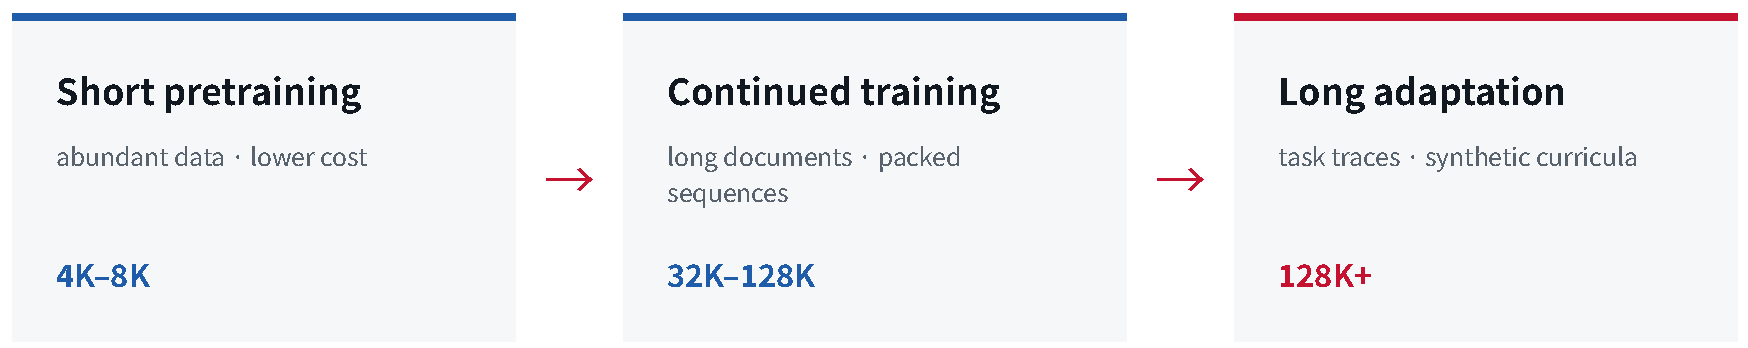
\includegraphics[width=\textwidth]{figures/从短预训练到长上下文适配.pdf}
\caption{长度逐步增长的训练路线。来源：官方课件第 27 页的矢量裁图；对应口述 00:35:57--00:37:41。}
\end{figure}

把多个短样本打包到一个长序列（packing）能够提高 token 利用率，也能让模型在靠后的位置接受训练。但若这些样本彼此独立，其答案不依赖其他样本的信息，训练并没有要求模型建立跨整个窗口的长程依赖。边界如何标识、是否隔离跨样本注意力，以及如何避免信息泄漏，都要由训练设计明确处理。

\begin{importantbox}{长度存在与长程依赖存在，需要分别检查}
一个 128K token 的批次可以由很多短文组成，也可以是一段从头到尾连贯的任务轨迹。这两者可能占用同样的上下文长度，却训练不同的行为。要学会长程检索、状态保持或跨文件推理，训练答案必须实际依赖远处的信息。
\end{importantbox}

\subsection{绝对位置、RoPE 与 NoPE：顺序信息从哪里进入模型}

\paragraph{绝对位置编码。}
最直接的做法，在 token 嵌入上加一个位置向量。位置因而在产生查询、键和值之前就进入模型。可学习位置表由一组离散向量组成；正弦编码则能按解析函数计算位置。

课件给出的输入和正弦编码为：
$$
\begin{aligned}
z_t&=E[x_t]+p_t,\\
p_{t,2\ell}&=\sin(t/\omega_\ell),
&p_{t,2\ell+1}&=\cos(t/\omega_\ell),
&\omega_\ell&=10000^{2\ell/d}.
\end{aligned}
$$
\begin{itemize}
  \item $t$：token 位置；$x_t$：该位置的 token ID；$E$：嵌入表；$z_t$：首层输入状态；$p_t$：位置向量。
  \item $d$：位置向量维数；$\ell$：正弦与余弦维度对的索引；$\omega_\ell$：该维度对的频率尺度。
  \item $p_{t,2\ell}$、$p_{t,2\ell+1}$：这一对位置向量分量；$\sin$、$\cos$：正弦与余弦函数；10000 是该方案的固定基数。
\end{itemize}

\paragraph{RoPE：用旋转把相对位移写入分数。}
旋转位置编码（Rotary Position Embedding, RoPE）对查询与键做位置相关的旋转。直观地看，两个向量都带上了各自位置的角度；做点积时，共同的旋转部分抵消，留下两者的相对位移。值向量不需要在这一机制中做同样的位置旋转。

\begin{figure}[H]
\centering
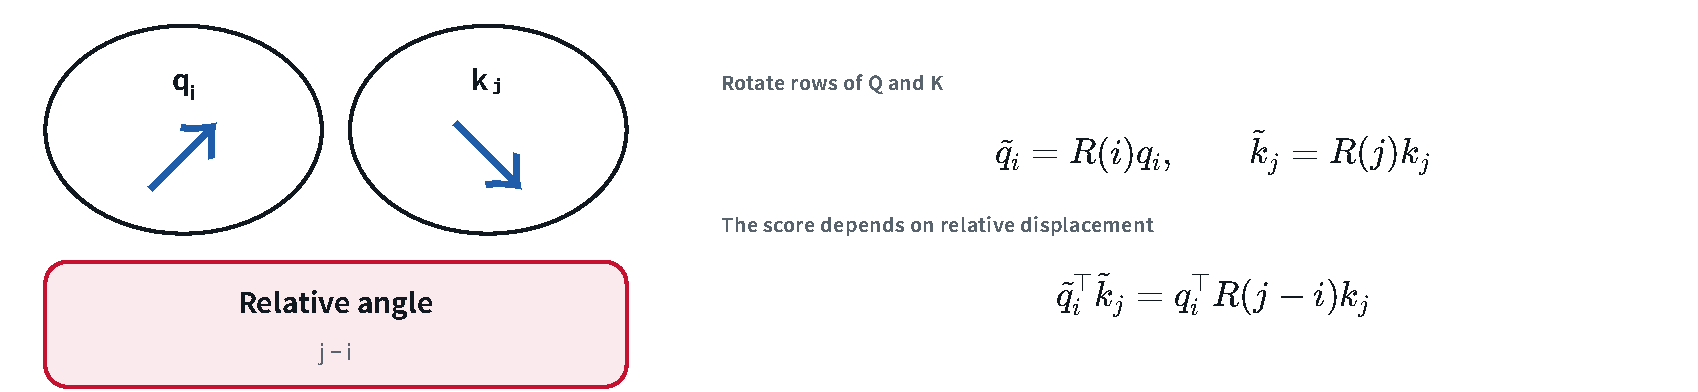
\includegraphics[width=\textwidth]{figures/RoPE的旋转与相对位移.pdf}
\caption{RoPE 将查询和键的旋转差转化为相对位移。来源：官方课件第 29 页的矢量裁图；对应口述 00:38:48--00:40:36。}
\end{figure}

以二维旋转构成块对角矩阵后，相对位置性质可写成：
$$
\widetilde q_i=R(i)q_i,
\qquad \widetilde k_j=R(j)k_j,
\qquad
\widetilde q_i^{\top}\widetilde k_j
=q_i^{\top}R(j-i)k_j.
$$
\begin{itemize}
  \item $i$、$j$：查询与键的位置；$q_i$、$k_j$：旋转前的内容向量；$\widetilde q_i$、$\widetilde k_j$：旋转后的向量。
  \item $R(t)$：由多组二维旋转组成的块对角矩阵，每组角度为 $t\theta_\ell$；$t$：旋转使用的位置或位移；$\theta_\ell$：第 $\ell$ 个二维块的每步旋转频率。
  \item $j-i$：本记号下的相对位移；$\top$：转置。关系使用旋转矩阵的正交性质，即 $R(i)^{\top}R(j)=R(j-i)$。
\end{itemize}

“相对”指这部分分数对位置的显式依赖通过相对位移进入。分数仍依赖查询与键的内容，模型的整体行为还受因果掩码和各层计算影响。因此，这个性质不能单独保证模型在从未训练过的长度上工作。

\paragraph{NoPE：不用显式位置编码，仍可以有顺序结构。}
NoPE 省去额外的位置向量与 RoPE 旋转。课堂问答指出，自回归模型的因果掩码本身就打破了所有位置的对称性：靠前的 token 只能看到较短前缀，靠后的 token 可以看到更长前缀。相同的词出现在不同位置，其可访问上下文不同，后续表示便可能不同。带有遗忘门的递推模型还通过更新顺序和衰减引入时间结构。

\begin{warningbox}{没有显式位置编码，不等于所有顺序都已自动学会}
因果计算或递推结构可以提供顺序信号，因此不能把全连接、无掩码情形中的置换对称直觉直接搬到自回归模型上。但 NoPE 仍需要训练长程行为，也不能保证任何重复 token 在任何输入上都一定得到不同表示。省去位置外推问题，并没有省去记忆容量、数据与泛化问题。
\end{warningbox}

\subsection{位置插值：将新位置映射回熟悉的相位范围}

若模型只在长度为 $L$ 的序列上受过训练，那么让它直接处理更远的相对距离，就会进入未见过的位置相位与注意力模式。统一位置插值的办法很直观：把更长序列的位置压缩回原来的相位范围。它改变的是\emph{RoPE 使用的位置坐标}，不会把实际 token 从序列中删除。

设目标长度是原长度的 $s$ 倍，课件的关系为：
$$
L'=sL,\qquad s=\frac{L'}{L},
\qquad
R(t)\longrightarrow R(t/s),
\qquad
\theta_\ell\longrightarrow\theta_\ell/s.
$$
\begin{itemize}
  \item $L$：原训练长度；$L'$：目标长度；$s$：扩展比例；$t$：目标序列中的实际位置。
  \item $R(t)$：原位置对应的 RoPE 旋转；$R(t/s)$：按压缩后的位置计算的旋转。
  \item $\theta_\ell$：第 $\ell$ 个旋转块的原频率；$\theta_\ell/s$：等价的缩小后频率。缩放坐标与缩放频率只需选择一种，不应重复做两次。
\end{itemize}

例如，从 8K 扩展到 32K 时，扩展比例为 4；位置 24000 在旋转计算中使用 6000。代价是相邻 token 在所有旋转维度中的相位间隔也一起缩小，局部位置区分可能变弱。插值因此通常还要配合适配训练与验证。

\subsection{YaRN：不同频率承担不同距离的区分}

统一压缩所有频率，可能同时损伤局部与全局位置的表达。YaRN 保留更多短波长、高频维度的局部相位，将长波长、低频维度充分插值，中间维度平滑混合。这样，距离扩展与局部区分可以分配给不同频率。

\begin{figure}[H]
\centering
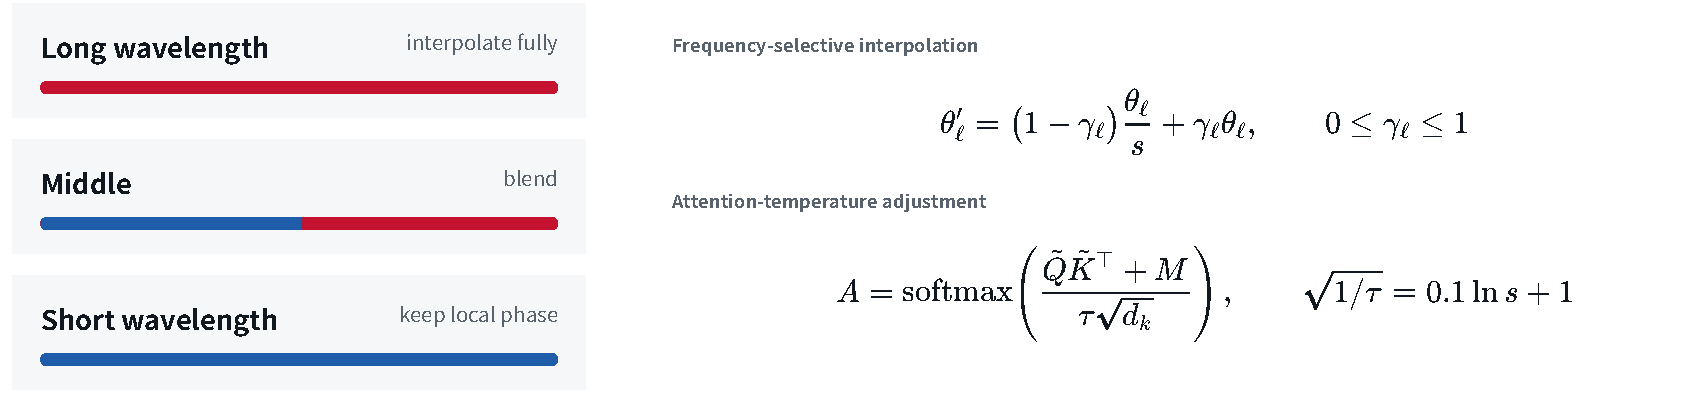
\includegraphics[width=\textwidth]{figures/YaRN的分频插值与温度.pdf}
\caption{YaRN 的长波长插值、短波长保留与温度修正。来源：官方课件第 32 页的矢量裁图；对应口述 00:45:30--00:46:14。}
\end{figure}

课件用下面的插值式概括这种分频选择：
$$
\theta'_\ell
=(1-\gamma_\ell)\frac{\theta_\ell}{s}
+\gamma_\ell\theta_\ell,
\qquad 0\le\gamma_\ell\le1.
$$
\begin{itemize}
  \item $\ell$：旋转维度对的索引；$\theta_\ell$、$\theta'_\ell$：原频率与调整后的频率；$s$：上下文扩展比例。
  \item $\gamma_\ell$：按波长选择的混合权重。长波长端取 0，进行完整插值；短波长端取 1，保留原频率；中间值混合两种行为。
\end{itemize}

YaRN 还调整注意力分数的温度，用来补偿扩展后注意力分布的变化。为了明确掩码角色，以下把温度作用写在内容分数上；因果掩码仍在屏蔽未来位置：
$$
A=\operatorname{softmax}\!\left(
\frac{\widetilde Q\widetilde K^{\top}}{\tau\sqrt{d_k}}+M
\right),
\qquad
\sqrt{1/\tau}=0.1\ln s+1.
$$
\begin{itemize}
  \item $A$：注意力权重矩阵；$\widetilde Q$、$\widetilde K$：经过调整后 RoPE 的查询与键矩阵；$\top$：转置；$d_k$：键维数。
  \item $\tau>0$：注意力温度；$M$：因果掩码，合法位置为 0，未来位置为负无穷；$\operatorname{softmax}$：对每个查询的候选键归一化。
  \item $s$：扩展比例；$\ln$：自然对数；$0.1$ 与 $1$：原论文经验拟合中的系数。
\end{itemize}

对这种 0/负无穷掩码，课件把掩码与分数一起除以正温度的写法具有相同屏蔽效果。温度公式是原论文在 LLaMA/Llama 2 系列上的经验配方，\textbf{并非适用于一切模型与长度的通用常数}。讲者只概括了 YaRN 的分频思路，温度的含义与上述边界来自课件及原论文的补充说明。

\subsection{模型案例：扩展位置与训练到长长度是不同安排}

课件列出的模型说明，达到大窗口可以有不同路径：采用部分 RoPE 的模型可能组合渐进训练与 YaRN；NoPE 模型无需重新缩放 RoPE，却仍要训练长距离任务；依靠 Mamba 递推或相对位置表示的模型则有各自的位置处理方式。下表按官方课件第 33 页概括\emph{课程材料中的实例}，用于比较机制。

\begin{table}[H]
\centering
\small
\begin{tabularx}{\textwidth}{@{}p{3.2cm}XX@{}}
\toprule
课件实例 & 位置信号 & 课件描述的扩展路线 \\
\midrule
Qwen3.8-Flash-Next & 部分 RoPE & 262K 原生窗口，结合 YaRN 扩展至 1M；完整训练课程未披露。 \\
DeepSeek V4 & 部分 RoPE & 4K、16K、64K、1M 渐进训练，并采用 YaRN。 \\
GLM-5.3-Flash & 主注意力采用 NoPE & 1M 原生窗口；无需 RoPE 重缩放，精确课程未披露。 \\
Kimi K3 & NoPE & 8K、64K、256K、1M 渐进训练。 \\
Nemotron 3 Ultra & Mamba 中的隐式顺序 & 进行 1M 长上下文继续预训练；监督微调长度到 512K。 \\
Inkling & 相对位置嵌入 & 1M 上下文；具体长度课程未披露。 \\
\bottomrule
\end{tabularx}
\caption{课件中的位置处理与训练路线实例。“未披露”保留了来源的信息边界；窗口值不等于全部任务都能可靠利用该长度。}
\end{table}

\subsection{数据：让答案真正依赖远处的证据}

讲者将长上下文训练的数据来源分成几类。它们的共同目标，是让模型在距离很远、伴随干扰信息的条件下，仍然保留任务需要的关联。

\begin{itemize}
  \item \textbf{自然长文档}：书籍、科学论文、技术报告等有连续结构的材料。优点是自然连贯，困难是足够长且高质量的资料数量有限。
  \item \textbf{代码库与多文档集合}：多个文件、议题、修改记录可以通过共同主题或工程依赖相连。讲者还提到专利等公共资料；把材料集合组织成任务仍需明确跨文档关系。
  \item \textbf{Agent 轨迹}：行动、工具观察、失败与恢复不断延长历史。训练可以要求模型追踪状态、记住约束，并使用很早以前的工具结果。
  \item \textbf{合成任务}：控制证据、干扰项和查询的位置，构造必须使用远处信息才能完成的任务。它们适合系统地覆盖长度，但不能仅凭合成任务成绩推出真实工作流程的表现。
\end{itemize}

按官方课件第 35 页，长数据与构造监督可以组合成不同配方：

\begin{table}[H]
\centering
\small
\begin{tabularx}{\textwidth}{@{}p{2.65cm}XX@{}}
\toprule
课件实例 & 自然材料 & 构造监督与长度安排 \\
\midrule
Kimi K3 & 清理、提高采样权重的文档及视频 & 重排多模态子任务，把证据铺到整个上下文；8K 到 1M 分阶段增长。 \\
GLM-5 & 文档、仓库文件、议题、PR 与差异文件 & 合成依赖与 Agent 轨迹；课件列出 32K、128K、200K。 \\
Nemotron 3\newline Ultra & 长文档问答 & 多文档推理、顺序扫描、合成表格；33B token 的 1M 继续预训练，监督微调到 512K。 \\
DeepSeek V4 & 科学论文与技术报告 & 长上下文预训练后进行 Agent 后训练；4K 到 1M 渐进增长。 \\
\bottomrule
\end{tabularx}
\caption{课程材料中的长上下文数据混合实例；此处保留可解释机制，不补造未披露的数据比例。}
\end{table}

讲者指出，公开权重的模型必须提供足够的结构信息才能运行，但数据混合与训练策略往往仍不完整公开。因此，这些实例能说明设计方向，不能据此复原某个模型的完整训练配方。

\begin{knowledgebox}{把“长依赖”变成可检验的数据设计}
可以先问：答案所需证据是否位于远处？是否必须组合多处证据？加入近处的错误候选后，模型还需要辨认正确来源吗？这些问题把“训练长序列”细化为可观察的行为。只增加填充内容或互不相干的短文本，不会自动产生上述要求。
\end{knowledgebox}

\subsection{上下文并行：把一个长序列分给多块设备}

长序列的激活和键值状态可能超过单块设备的承载能力。上下文并行（context parallelism）把\emph{同一个序列的位置维度}划分到多个设备。它与把不同样本分给设备的数据并行、把参数或层分给设备的模型并行处理不同维度，也可以组合使用。

以课件的 Ring Attention 示意为例，每个设备持有一部分查询，键值块在设备之间流转。设备针对自己的查询累积各个键值块的注意力计算，再发送或接收下一块。计算可以与通信重叠；因果约束仍需要在块级计算中保持。

\begin{figure}[H]
\centering
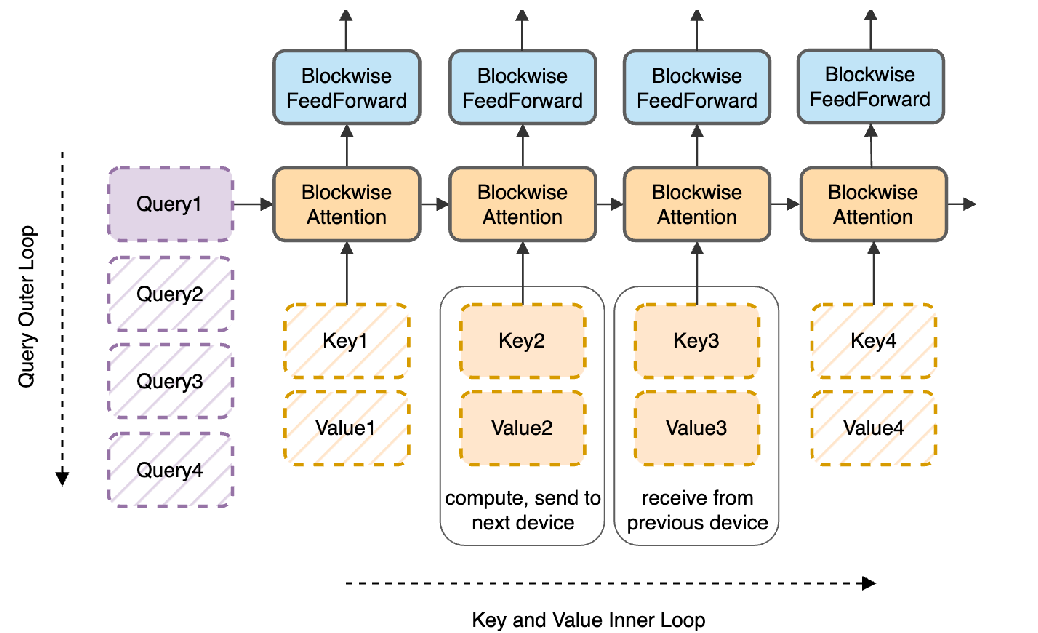
\includegraphics[width=0.78\textwidth]{figures/上下文并行的查询与KV分块.pdf}
\caption{查询分块与键值块传递的上下文并行示意。来源：官方课件第 36 页的矢量裁图；对应口述 00:48:56--00:52:06。}
\end{figure}

课件给出的阶数关系说明它解决的是分布式存储和执行问题：
$$
\text{每设备相关状态规模}
=O\!\left(\frac{nd_k}{P}\right),
\qquad
\text{稠密注意力总工作量}=O(n^2d_k).
$$
\begin{itemize}
  \item $n$：总序列长度；$d_k$：键维数，课件以此概括每位置表示尺度；$P$：参与上下文划分的设备数量。
  \item $O(\cdot)$：忽略固定维度、常数及实现细节后的增长阶数；“相关状态”不包括整套模型权重与全部训练开销。
\end{itemize}

\begin{warningbox}{上下文并行没有把稠密注意力变成线性算法}
分块、传递与重叠执行可降低每块设备需要持有的状态，并使长序列能够跨设备计算；全局的稠密配对工作仍保持二次增长。通信带宽、块调度、在线归一化与反向传播也会影响速度。不能直接把所有设备的局部 softmax 输出相加：跨块结果必须正确合并其归一化信息。
\end{warningbox}

最后还有架构与基础设施的兼容性。讲者讲述自己尝试为一种 Gated DeltaNet 模型做上下文并行时，遇到可用内核不足的问题。标准注意力的成熟实现不能直接代替另一种递推更新所需的并行与反向传播内核。这是课堂中的工程经验：选择模型结构时，除了理论复杂度，也要检查所用训练系统能否正确支持它。

\subsection{本章小结}
\begin{itemize}
  \item 训练长度可以逐步增长，但样本打包和跨全文依赖提供的训练信号不同。
  \item 绝对位置编码将位置加进输入；RoPE 用查询与键的旋转表达相对位移；NoPE 可以依靠因果或递推结构获得顺序信号。
  \item 统一位置插值缩放 RoPE 的相位坐标；YaRN 按频率选择插值强度，并采用有适用范围的温度修正。
  \item 连贯长资料、Agent 轨迹和合成监督应让答案实际依赖远处证据，而不只是让输入变长。
  \item 上下文并行减少每设备负担，仍需支付稠密总计算与跨设备通信成本，并受模型内核支持情况约束。
\end{itemize}

\subsection{拓展阅读}
\begin{itemize}
  \item \href{https://arxiv.org/abs/2309.00071}{Peng 等：YaRN}，详细说明分频插值、注意力温度与适配实验。
  \item \href{https://arxiv.org/abs/2310.01889}{Liu 等：Ring Attention}，介绍分块计算与通信重叠的长序列执行方式。
\end{itemize}


\clearpage
\section{Prompt 与 KV 缓存：复用已经完成的计算}

架构和长上下文训练解决了“模型怎样处理长历史”的问题。Agent 的实际调用还有一个特点：相邻两轮的输入往往高度重合。上一轮的系统指令、用户要求、模型动作和工具结果，通常仍在下一轮历史里。如果每一轮都从头计算这些内容，系统会反复为同一段历史支付预填充成本。缓存要利用的正是这部分重合。

\subsection{一轮内的 KV 扩展与多轮之间的前缀复用}

先区分两个时间尺度。在\textbf{一次模型调用内}，prefill 为输入位置建立 KV；随后逐 token decode，新生成 token 的 KV 继续加入缓存，供后续 token 使用。在\textbf{连续模型调用之间}，服务系统还可以保留这些已经计算好的状态，让下一次输入中完全相同的前缀直接复用。

工具结果是两轮之间的新增信息。模型输出工具调用时，还没有读到外部执行结果，因此下一轮必须先处理新返回的结果。处理完后，这部分也能加入未来可复用的历史前缀。下图从 Call 1 到 Call 3 逐步增加蓝色缓存区，同时保留每轮新增的红色输入、黑色输出和灰色工具结果。

\begin{figure}[H]
\centering
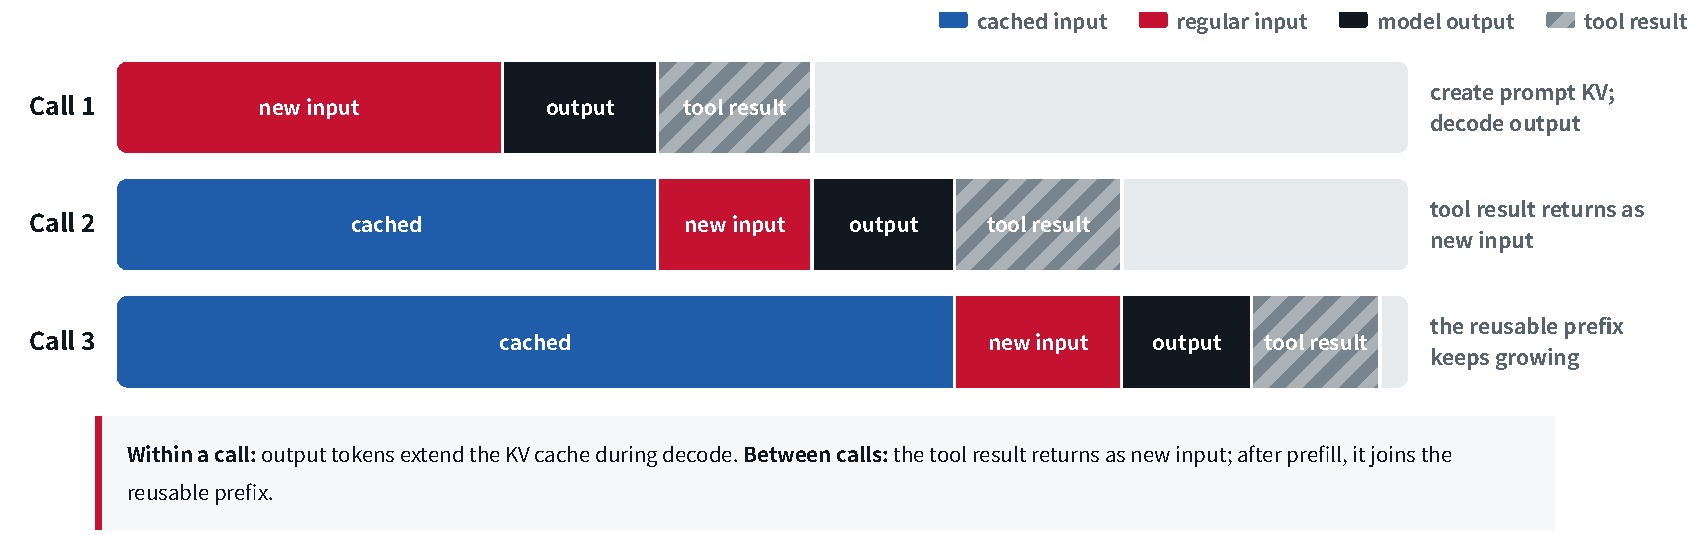
\includegraphics[width=\textwidth]{figures/缓存前缀随Agent循环增长.pdf}
\caption{官方课件第 38 页：Agent 循环中的可复用前缀持续增长。\newline{\footnotesize 对应口述 00:52:06--00:54:50。}}
\end{figure}

\begin{importantbox}{缓存保存的是计算状态，历史仍然可见}
命中前缀缓存后，系统可省去旧前缀的重复 prefill；模型继续生成时，仍需使用旧前缀的 KV 来执行注意力。缓存没有删掉旧 token，也没有缩短模型可见的上下文，因此它不能单独解决上下文窗口上限或历史增长带来的 KV 容量问题。
\end{importantbox}

“同样的文本”也需要放在正确的计算条件下理解。普通因果模型某位置的 KV 依赖其前面的内容；相同句子若出现在不同前缀之后，其状态未必相同。复用通常要求兼容的模型、分词、位置和请求配置，并匹配同一段前缀。Prompt Cache 论文进一步研究了显式定义的可复用模块及其位置管理；这比把任意同义文本视为同一缓存项严格得多。

\subsection{为什么读取缓存会比重新计算便宜}

重复 prefill 要重新运行注意力和前馈网络等计算；缓存命中则复用已经得到的状态。读取和传输状态仍有开销，所以收益要看历史长度、硬件、带宽和存储位置。课件中的 Prompt Cache 实验把重新计算与缓存读取放在一起比较：同一种硬件的两条曲线应成对阅读，缓存开始占优的位置随硬件而变化。

\begin{figure}[H]
\centering
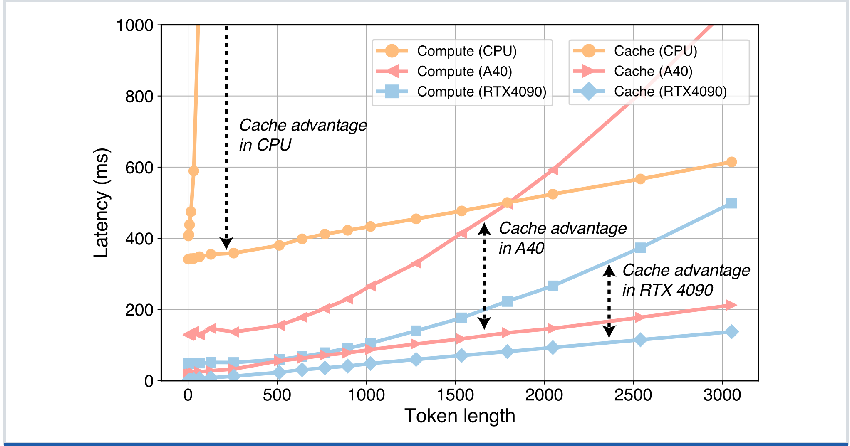
\includegraphics[width=0.88\textwidth]{figures/缓存读取与重新计算的时延.pdf}
\caption{官方课件第 39 页 左图：随着 token 长度增加，重新计算与缓存读取的时延差异扩大；收益拐点依硬件而变。\newline{\footnotesize 对应口述 00:53:24--00:54:50。}}
\end{figure}

讲者用“未缓存计算增长更快，缓存读取更接近线性”解释图形趋势。这个说法描述该图的工作负载与测量范围；它不意味着一次缓存命中会让整个 Agent 的所有计算变为线性，更不意味着 decode 不再随可访问历史增长而变贵。

另一种收益来自\textbf{摊销}：同一段文档先做一次 prefill，再由许多调用复用它，首次建立状态的开销可以分摊到这些调用上。课件右图横轴是复用次数，纵轴是摊销后的每次物理成本；多次复用后，曲线逐渐接近复用本身的成本下界。

\begin{figure}[H]
\centering
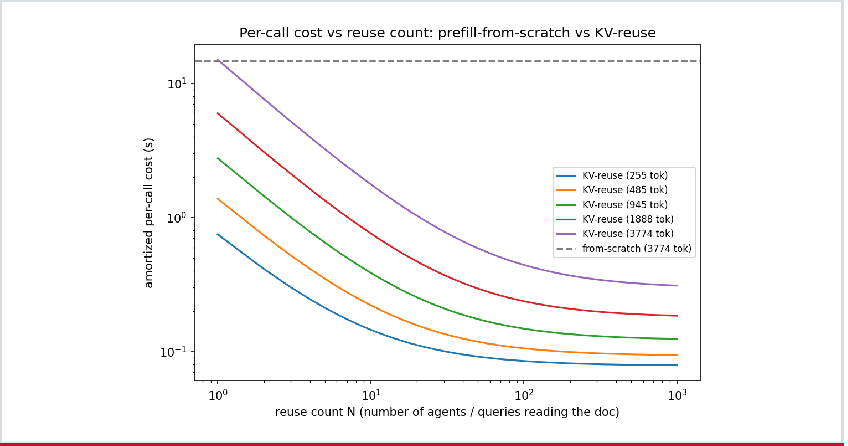
\includegraphics[width=0.88\textwidth]{figures/KV预填充成本的多次复用.pdf}
\caption{官方课件第 39 页 右图：一次预填充成本可被多次读取摊销，曲线最终趋近每次复用的成本。\newline{\footnotesize 对应口述 00:53:24--00:54:50。}}
\end{figure}

\begin{knowledgebox}{物理成本与 API 价格属于不同层面}
物理成本讨论计算、内存、传输和设备时间。API 价格还包含供应商的定价与计费规则。实验中缓存节约了多少计算，与账单中缓存 token 打几折，不能直接互相替代。
\end{knowledgebox}

\subsection{缓存 token 的价格与命中率}

课件 P40 给出了\textbf{2026 年 8 月 30 日核对的课堂价格快照}，单位为每百万 token 的美元金额。“Cached input”指缓存读取命中；缓存创建有可能另计。DeepSeek 的区间表示课件列出的低峰与高峰价格。

\begin{table}[H]
\centering
\small
\begin{tabularx}{\textwidth}{L{3.5cm} L{2.7cm} L{2.7cm} X}
\toprule
课件中的模型 & 缓存输入 & 普通输入 & 输出 \\
\midrule
DeepSeek V4 Flash & \$0.007--0.014 & \$0.22--0.44 & \$0.66--1.32 \\
GLM-5.2 & \$0.26 & \$1.40 & \$4.40 \\
Kimi K3 & \$0.30 & \$3.00 & \$15.00 \\
GPT-5.6 Luna & \$0.02 & \$0.20 & \$1.20 \\
GPT-5.6 Sol & \$0.40 & \$4.00 & \$20.00 \\
Claude Opus 5 & \$0.50 & \$5.00 & \$25.00 \\
\bottomrule
\end{tabularx}
\caption{官方课件第 40 页 的历史价格快照，保留课堂比较所用的数值。}
\end{table}

表里若干模型的缓存读取价格为普通输入的十分之一；各行的比例并不完全相同。讲者又指出输出往往比普通输入贵，因此维护缓存、避免无用输出，对账单都有明显影响。例如当输出价格恰为普通输入的五倍，而缓存输入恰为十分之一时，输出与缓存输入的单价相差五十倍。这是满足这两个条件的比例计算。

为看清这三个计费部分，可作如下\textbf{教学推导}。一次调用的历史命中了多少缓存、新增多少输入、生成多少输出，分别乘上对应单价，再相加；暂不计缓存创建、存储或其他费用。
$$
C_{\mathrm{call}}=\frac{p_c H+p_u U+p_o V}{10^6}
$$
\begin{itemize}
\item $C_{\mathrm{call}}$：该调用的美元费用。
\item $p_c$：每百万缓存命中输入 token 的价格。
\item $H$：本轮按缓存读取计费的输入 token 数。
\item $p_u$：每百万普通输入 token 的价格。
\item $U$：本轮按普通输入计费的 token 数。
\item $p_o$：每百万输出 token 的价格。
\item $V$：本轮输出 token 数。
\item $10^6$：将 token 数换算成“每百万 token”计价单位。
\end{itemize}

再以输入 token 为单位定义命中率，就能把“有几次请求命中”和“总共节约了多少前缀重算”区分开。
$$
h=\frac{H}{H+U},\qquad
p_{\mathrm{input,avg}}=h p_c+(1-h)p_u
$$
\begin{itemize}
\item $h$：本轮输入 token 的缓存命中比例，假设 $H+U>0$。
\item $H$：缓存命中的输入 token 数。
\item $U$：未按缓存命中计费的输入 token 数。
\item $p_{\mathrm{input,avg}}$：按本轮输入组成加权的每百万 token 平均单价。
\item $p_c$：每百万缓存输入 token 的价格。
\item $p_u$：每百万普通输入 token 的价格。
\end{itemize}

若 $p_c=p_u/10$，命中率为 90\% 时，平均输入单价为 $0.19p_u$；95\% 时为 $0.145p_u$。这些数值只描述输入部分，不能直接当成整项任务的总成本降幅。讲者把 90\%--95\% 视为自己运行 Agent 时较满意的经验范围；具体合理值还取决于工作负载和服务端的统计口径。

\subsection{PagedAttention：逻辑连续，物理分块}

KV cache 会随着每个请求生成而增长，不同请求又在不同时间结束。若为每个请求预留一大块连续显存，会浪费未使用空间，也容易受到碎片影响。PagedAttention 借鉴分页思想，把一个序列的 KV 分成固定大小的逻辑块，通过块表映射到物理 GPU 内存块。

\begin{figure}[H]
\centering
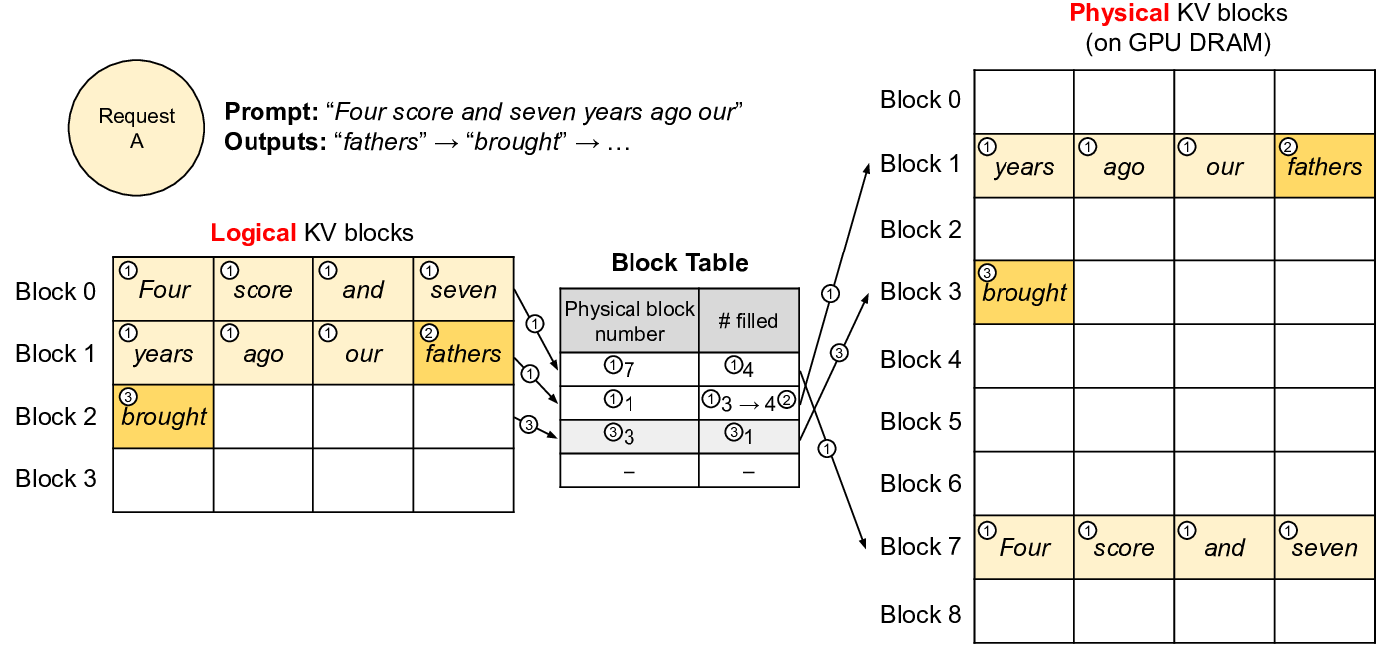
\includegraphics[width=0.93\textwidth]{figures/PagedAttention逻辑块与物理块.pdf}
\caption{官方课件第 41 页：逻辑 KV 块经块表映射到分散的物理显存块。\newline{\footnotesize 对应口述 00:57:26--00:58:20。}}
\end{figure}

图中逻辑 Block 0、1、2 分别放在物理 Block 7、1、3。逻辑顺序保持连续，物理位置可以不连续。随着输出从 \texttt{fathers} 增长到 \texttt{brought}，已有块继续填充，必要时再分配新块。多个请求结束时，系统可以按块回收和再分配空间，支持更高效的并发服务。

这个机制主要改变\textbf{KV 的存储组织和访问方式}。它不负责决定哪些历史可以语义性丢弃，也不自动缩短每个请求需要关注的历史。

\subsection{RadixAttention、路由与缓存淘汰}

有了分块存储，还需要快速回答“新请求与哪些已缓存请求共享前缀”。RadixAttention 使用基数树组织前缀：相同部分共享树路径，分歧部分形成不同分支。课件展示了三个核心操作。

\begin{figure}[H]
\centering
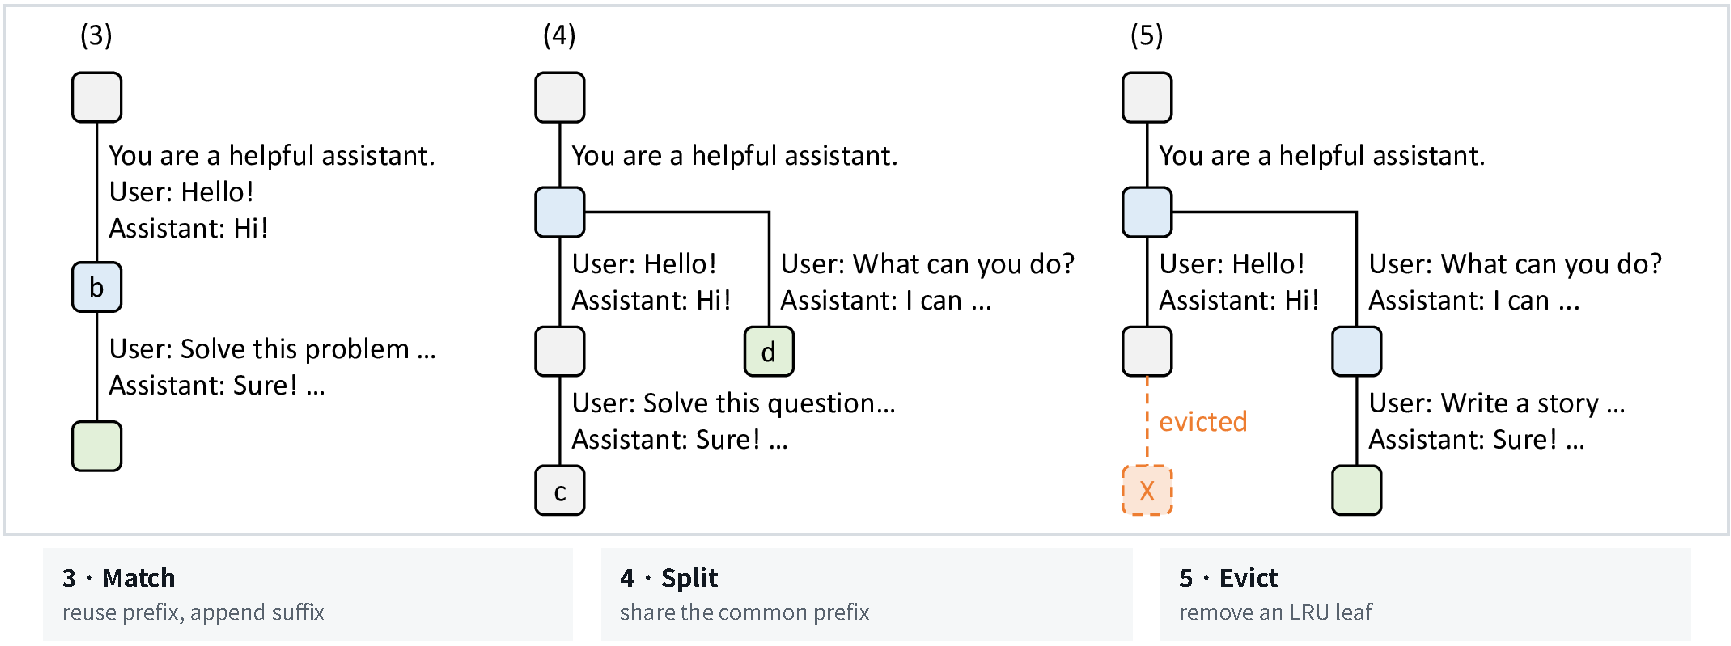
\includegraphics[width=\textwidth]{figures/RadixAttention匹配分裂与淘汰.pdf}
\caption{官方课件第 42 页：匹配已有前缀、在分歧位置分裂，以及淘汰较久未使用的叶节点。\newline{\footnotesize 对应口述 00:58:20--00:59:46。}}
\end{figure}

\begin{enumerate}
\item \textbf{Match}：找到可复用的前缀，只为后续新增部分建立状态。
\item \textbf{Split}：请求共享开头但后来分岔时，把共同部分保留为共享路径，再创建不同的后缀分支。
\item \textbf{Evict}：显存有限，优先移除可以回收的旧缓存；图中展示较久未使用叶节点的淘汰。
\end{enumerate}

多机器服务还多了一层选择：同一个请求发给哪一台机器。纯负载均衡可能把它送到空闲但没有历史缓存的 worker。缓存感知路由则同时估计可复用前缀和排队负担，让已经拥有相关 KV 的 worker 有机会继续服务。

\begin{figure}[H]
\centering
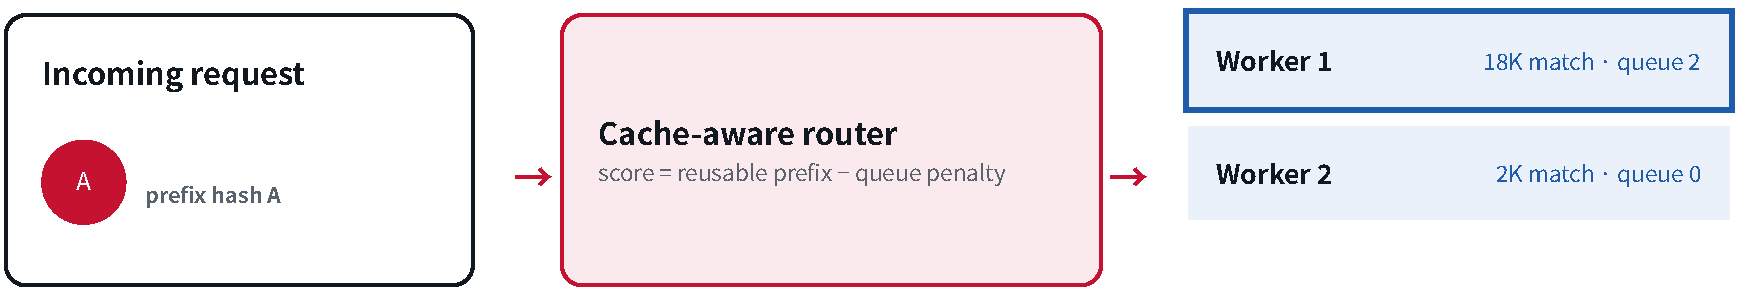
\includegraphics[width=\textwidth]{figures/缓存感知路由.pdf}
\caption{官方课件第 43 页：路由同时考虑可复用前缀与队列负担。图中的减法是评分思想示意。\newline{\footnotesize 对应口述 00:59:46--01:00:32。}}
\end{figure}

图里 Worker 1 有 18K 前缀匹配但队列里有两个请求，Worker 2 只有 2K 匹配而队列为空。最终选择取决于重算节约能否抵消等待。图中“可复用前缀减队列惩罚”不提供具体单位换算或权重，不能直接把 token 数与队列长度相减作为通用生产公式。

缓存命中还受\textbf{淘汰策略}影响。提供方不会永久保存每个会话的 KV；空闲时间、显存压力和保留策略都可能让本来相同的前缀失去命中。讲者展示的提供方比较也可能混入不同工作负载，不能只凭命中率判断服务实现优劣。课堂关于分钟级或小时级保留，以及 GPU 到 CPU 的缓存转移，属于当时的经验与问答，具体保留期限和分层方式由服务实现决定。

\subsection{Harness 如何保持稳定前缀}

即使不部署模型，Harness 也会通过请求构造影响缓存。最简单的原则是：\textbf{稳定信息放前面，变化状态追加到后面}。系统指令、工具定义和固定示例需要稳定的内容与顺序；新用户消息、当前时间、最新工具观察则随轮次追加。

下面是根据课堂原则整理的教学示意，展示消息布局，不绑定某一家 SDK。它把同一段系统说明保留在开头，把每轮更新的时间放在末尾的新观察里。

\noindent\begin{minipage}{\textwidth}
\begin{lstlisting}[language=Python,caption={教学示意：固定系统前缀，追加变化的运行状态}]
system_message = {"role": "system", "content": stable_instructions}
request_messages = [system_message, *prior_messages]
request_messages.append({
    "role": "user",
    "content": f"Current time: {now}. Latest observation: {observation}"
})
\end{lstlisting}
\end{minipage}

如果把时间戳改写进最前面的系统消息，两轮请求可能从很早的位置就出现分歧，后面即使有大量相同文本，也失去普通前缀缓存的条件。动态工具同样要看它们在请求序列中的位置：增删工具、改变 Schema 或改变工具排序若改动了前部 token，就可能缩短可复用前缀。

\begin{warningbox}{模型切换的节约要算上缓存状态}
不同模型的 KV 通常不能直接共用。切到便宜模型后再切回原模型，需要检查原模型一侧还有多少可复用前缀、缓存是否被淘汰，以及中间新增历史是否已处理。不能只比较单 token 标价，就假定频繁切换会降低整个会话的费用。
\end{warningbox}

\subsection{本章小结}

\begin{itemize}
\item 一轮内的 KV cache 支撑逐 token 生成，多轮之间的前缀缓存省去相同历史的重复 prefill。
\item PagedAttention 管理物理内存块；RadixAttention 找到共享前缀；缓存感知路由和淘汰策略决定这些状态能否被再次利用。
\item 输入 token 命中率、首 token 时延、缓存保留和实际账单需要一起观察。
\item 缓存收益依赖稳定的精确前缀；它保留历史可见性，并不代替上下文压缩。
\end{itemize}

\subsection{拓展阅读}

\begin{itemize}
\item \href{https://arxiv.org/abs/2309.06180}{PagedAttention / vLLM}：理解动态增长的 KV 如何分页、共享和回收。
\item \href{https://arxiv.org/abs/2312.07104}{SGLang}：理解基数树前缀复用及其与多次调用程序的关系。
\end{itemize}

\clearpage
\section{上下文压缩：为后续动作保留任务状态}

缓存能减少反复计算，但 Agent 的历史仍会增长。当历史超出预算，系统需要决定哪些内容直接保留、哪些内容浓缩、哪些证据转移到外部、哪些内容可以舍弃。Context compaction 的核心困难是：压缩后仍要继续执行同一项任务，已有约束、确认结果和外部动作不能被随意改写。

\subsection{从长轨迹到可继续工作的状态}

课件使用一个 CI 超时示例。原始轨迹记录：任务超时、检查日志、发现大量端口占用错误、设置 \texttt{--workers=1}、测试通过并保存日志。浓缩后保留下列信息：修复目标、端口冲突这一原因、已验证的配置、证据路径，以及下一项动作。

\begin{figure}[H]
\centering
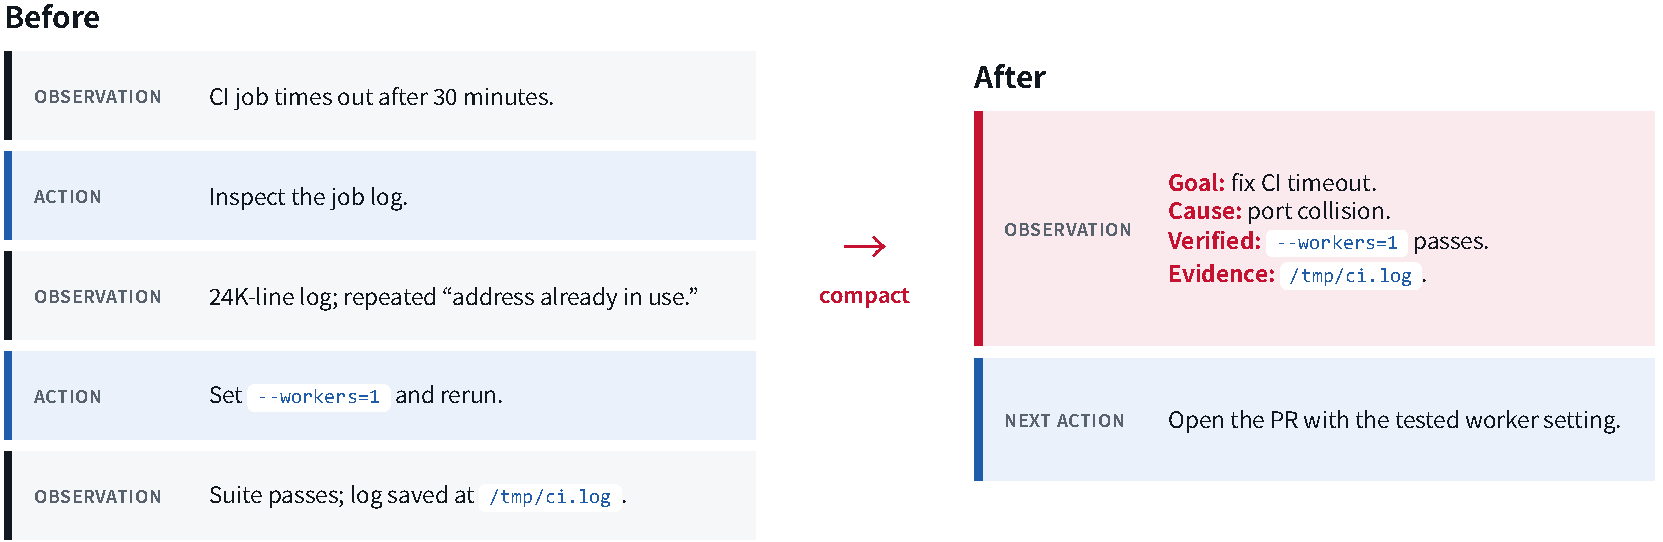
\includegraphics[width=\textwidth]{figures/CI任务压缩前后状态.pdf}
\caption{官方课件第 46 页：压缩后的状态保留目标、诊断、已验证结果和证据位置。\newline{\footnotesize 对应口述 01:06:23--01:08:01。}}
\end{figure}

这个示例中，提交 PR 被标为\textbf{下一项动作}，而“测试通过”是\textbf{已经完成的动作结果}。两者若在压缩时混淆，Agent 可能重跑已完成工作，也可能重复提交。能继续行动的状态必须保留这些状态差别。

\begin{importantbox}{压缩质量由后续行为检验}
一份摘要能否让人读懂只是起点。好的工作状态还应让 Agent 知道当前目标、必须满足的条件、已经做过什么、哪些结果经过验证、哪里能找回证据，以及接下来应做什么。
\end{importantbox}

\subsection{把 compaction 看成状态估计}

课件 P47 把压缩写成从完整历史估计工作状态。直觉是：在一个有限预算中构造较短表示，让基于它做出的未来动作，与基于完整历史做出的动作尽可能一致。这个目标要求\textbf{行为保真、表示有界和证据可恢复}三者同时考虑。
$$
\hat{s}_t=\mathcal{C}(H_t;B),\qquad
|\hat{s}_t|\leq B,\qquad
p(A_{\mathrm{future}}\mid H_t)\approx
p(A_{\mathrm{future}}\mid\hat{s}_t)
$$
\begin{itemize}
\item $\hat{s}_t$：时间 $t$ 的压缩后工作状态。
\item $t$：当前历史所处的时间或任务步。
\item $\mathcal{C}$：上下文压缩过程。
\item $H_t$：截至时间 $t$ 的完整历史。
\item $B$：压缩后工作状态的 token 预算。
\item $|\hat{s}_t|$：工作状态的 token 长度。
\item $p$：未来动作序列的条件分布。
\item $A_{\mathrm{future}}$：后续动作序列。
\item $\approx$：希望行为尽可能相近；这是设计目标，不能视作已证明的等价关系。
\end{itemize}

有限状态无法无损保留任意长历史的全部细节。要判断哪些信息可以浓缩，必须结合任务：某段日志的二万四千行可能可以移出当前上下文，但用户规定的精确版本号、当前分支、已经创建的 PR 编号，往往需要原样保留。

\subsection{锚点、检查点、最近尾部与外部证据}

课件 P48 给出一种分工：目标与约束作为锚点，进展与决定编码为检查点，最近仍在活动的尝试保留为尾部，长证据存入外部，重复或已被替代的内容可以舍弃。

\begin{figure}[H]
\centering
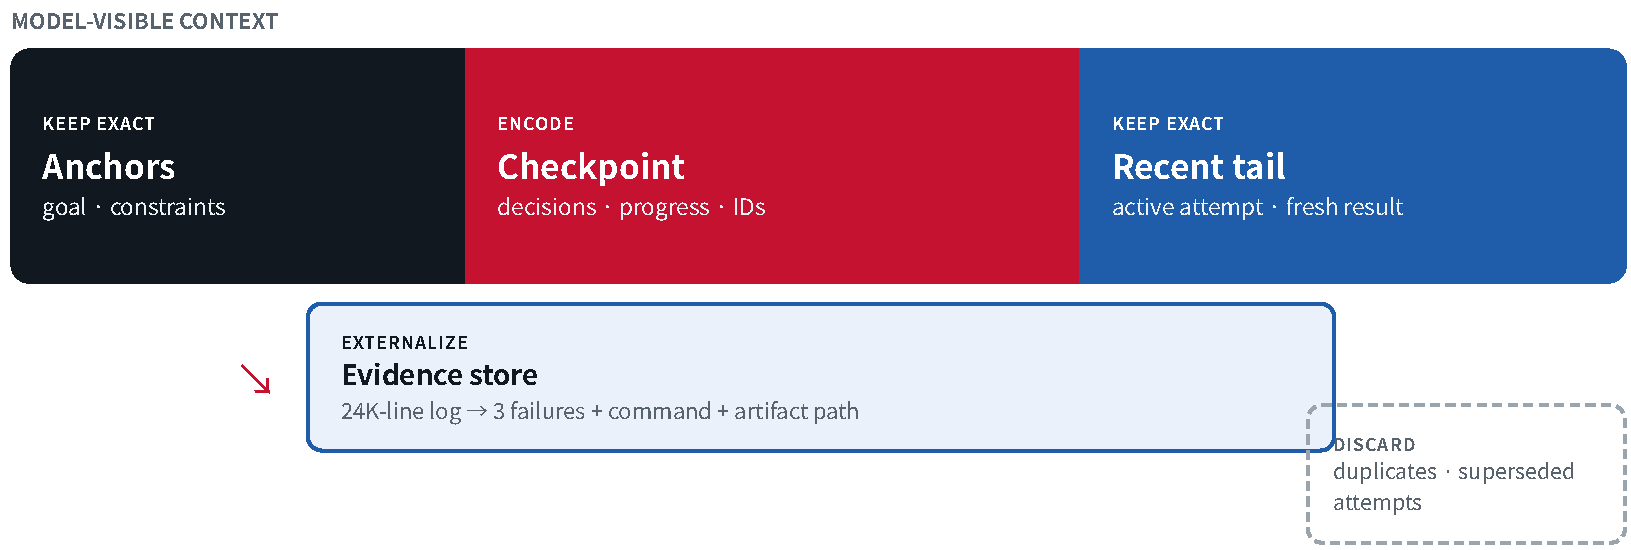
\includegraphics[width=\textwidth]{figures/压缩后的锚点检查点与证据.pdf}
\caption{官方课件第 48 页：不同类型的信息采用原样保留、状态编码、外部化或舍弃。\newline{\footnotesize 对应口述 01:08:01--01:10:15。}}
\end{figure}

\begin{itemize}
\item \textbf{Anchors（锚点）}：精确目标、用户约束、必须遵守的条件。开头常常包含这些信息，但后续用户修正也可能形成新锚点。
\item \textbf{Checkpoint（检查点）}：已作决定、当前进度、完成与待办事项、关键标识符。它让 Agent 从正确位置继续。
\item \textbf{Recent tail（最近尾部）}：当前尝试、刚返回的工具结果、仍待处理的错误；保留它有助于维持局部动作连续性。
\item \textbf{Evidence store（证据存储）}：原始日志、检索结果、长轨迹或其他产物。上下文内保留能定位它们的路径、查询或标识符。
\item \textbf{Discard（舍弃）}：重复内容和被后续结果明确替代的尝试；舍弃需要确认它们已无后续作用。
\end{itemize}

“保留开头”是一种常见策略，不能替代“保留当前有效要求”。用户在会话中途更新目标时，检查点也必须更新。证据外部化则依赖真实可访问的存储和检索路径：只写“可查原始记录”而没有位置或工具，并不能让 Agent 恢复证据。

下面的结构化检查点是\textbf{教学补充}，将课件的 CI 示例编码成可审查的字段。它展示状态内容，不规定通用格式；真实系统还需要验证字段与原始记录一致。

\noindent\begin{minipage}{\textwidth}
\begin{lstlisting}[language={},caption={教学示意：保留已验证结果和未完成动作的结构化检查点}]
{
  "goal": "Fix the CI timeout",
  "constraints_exact": ["Keep the tested worker setting"],
  "diagnosis": "Port collision",
  "verified": [
    {"setting": "--workers=1", "result": "Suite passes"}
  ],
  "evidence": ["/tmp/ci.log"],
  "external_actions_done": [],
  "next_action": "Open the PR with the tested setting"
}
\end{lstlisting}
\end{minipage}

\subsection{压缩策略要回答四个问题}

压缩不是一条“请总结以上内容”的提示就能定义完整。课件 P49 把过程拆成触发、选择、替换与恢复四项策略。

\begin{figure}[H]
\centering
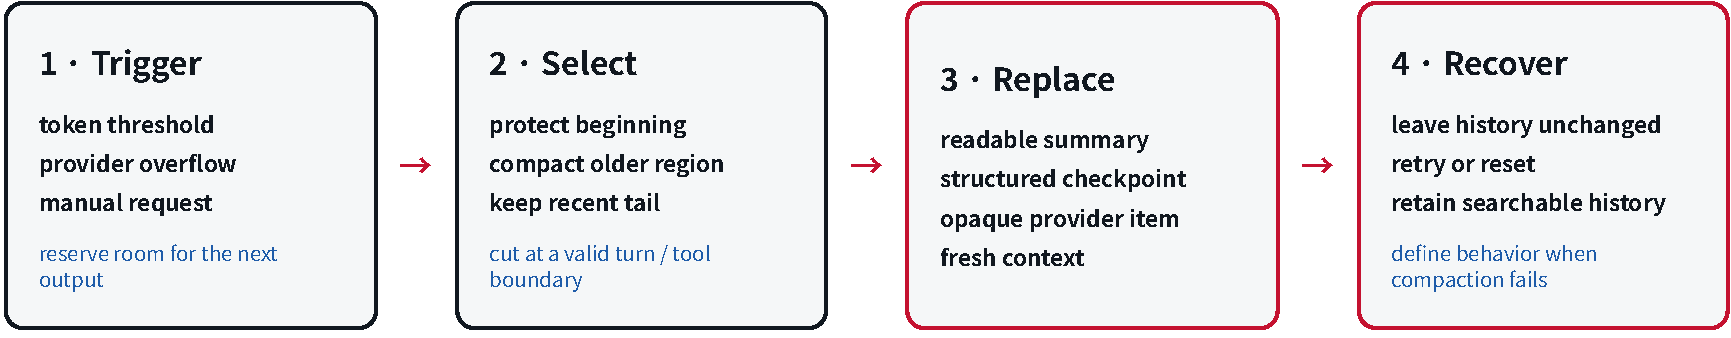
\includegraphics[width=\textwidth]{figures/上下文压缩的四项策略.pdf}
\caption{官方课件第 49 页：完整的压缩策略需要定义触发、选区、替换表示和失败恢复。\newline{\footnotesize 对应口述 01:10:15--01:12:01。}}
\end{figure}

\textbf{第一，何时触发？}可以采用 token 阈值、提供方的上下文硬上限，或人工请求。讲者举出的 200K 阈值是说明策略的例子。系统还需要给下一轮输出留空间；若一直等到完全塞满，压缩请求本身或下一次动作也可能没有预算。

\textbf{第二，选哪一段？}常见做法是保护锚点和最近尾部，压缩较旧的中间区域。截断点还要维持有效的会话结构。尤其是工具调用与对应结果，不能被任意切开后留下无法理解的片段。

\textbf{第三，用什么替换？}可以用自然语言摘要、结构化检查点，或提供方支持的不透明压缩项。课堂提到的不可读压缩项减少了用户直接查看其内容的能力；其格式与处理规则由提供方决定，不能假定可以移植成通用明文摘要，也不能据此保证完整历史可以恢复。

\textbf{第四，失败后怎样处理？}要定义压缩调用失败、结果不合格或上下文仍超预算时的行为，例如保留原历史并重试，或从可检索历史建立新状态。系统应在新状态准备好后再替换旧工作上下文，并保留必要的回退证据。保留旧历史并不代表在硬上限处可以不经处理直接继续调用。

\begin{warningbox}{压缩不能抹掉仍然有效的动作边界}
如果一项工具调用尚未收到结果，应把它作为待完成状态保存；如果一次外部提交已经成功，应保存完成事实与对象标识符。压缩后把“已完成”写成“下一步”，可能导致重复执行有副作用的动作。
\end{warningbox}

\subsection{反复压缩会累积漂移}

一次摘要已经丢掉的细节，下一次摘要通常无法凭空找回来。课件用版本约束展示这种累积：\texttt{CUDA 12.4} 先被概括成 \texttt{CUDA 12.x}，再变成“较新的 CUDA”，最后约束消失。

\begin{figure}[H]
\centering
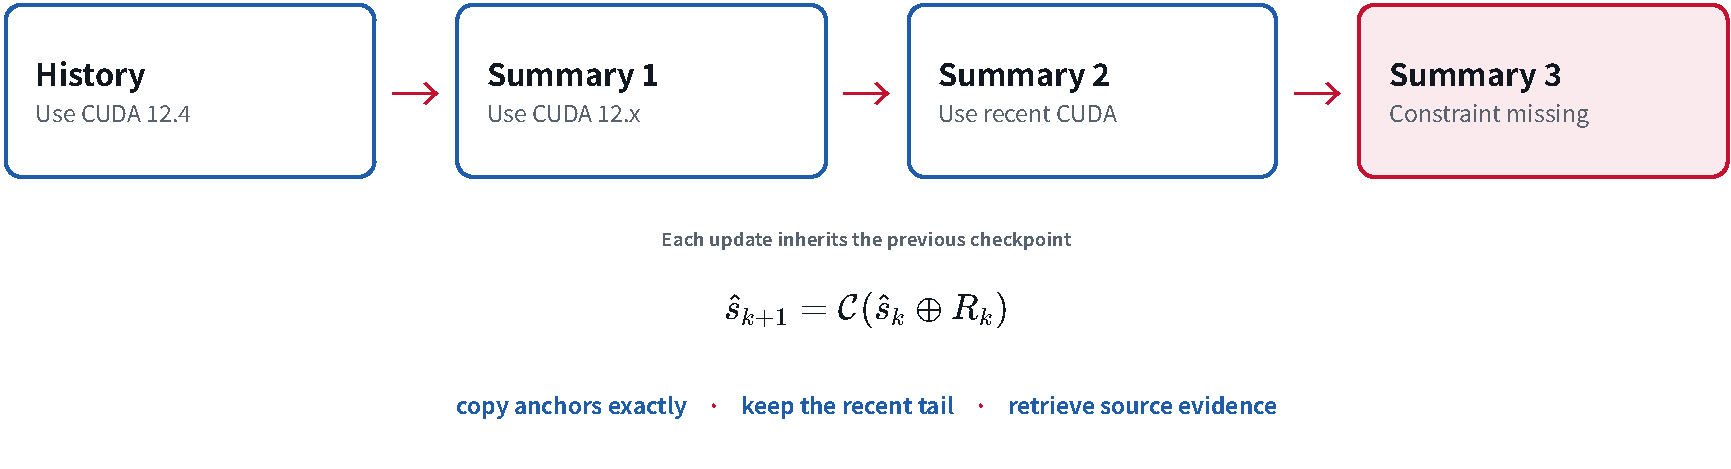
\includegraphics[width=\textwidth]{figures/重复压缩的约束漂移.pdf}
\caption{官方课件第 50 页：逐次转述可能逐步削弱精确约束。\newline{\footnotesize 对应口述 01:12:01--01:14:03。}}
\end{figure}

每次更新如果只拿“旧检查点加最近新轨迹”再压缩，就会继承旧检查点的遗漏。这可以写成以下更新关系。
$$
\hat{s}_{k+1}=\mathcal{C}(\hat{s}_k\oplus R_k)
$$
\begin{itemize}
\item $\hat{s}_{k+1}$：下一次压缩后的工作状态。
\item $\mathcal{C}$：压缩过程。
\item $\hat{s}_k$：第 $k$ 次压缩得到的旧工作状态。
\item $k$：压缩次数的索引。
\item $\oplus$：按相应会话格式组合旧状态和新增记录。
\item $R_k$：上一次压缩后新增的轨迹。
\end{itemize}

缓解方法与前面的信息分工一致：精确锚点直接复制；关键状态字段保持可审查；保留最近活动尾部；对有歧义的决定回查原始证据。一个版本号若从一开始就被替换成模糊描述，只靠再次总结无法补回精度。

\subsection{评价必须让 Agent 压缩后继续执行}

讲者分享了 OpenHands 早期的经验：团队设计的压缩方法在代码任务基准上保持成绩，又节约了大量 token，但用于真实交互后出现了新问题。它可能忘记已经向 GitHub 提交过 PR，于是反复提交同一功能；也可能忘掉会话中途的用户指令，因为原先评测主要覆盖只有一次用户消息的任务。这个故事指出了\textbf{评测分布的缺口}。

\begin{figure}[H]
\centering
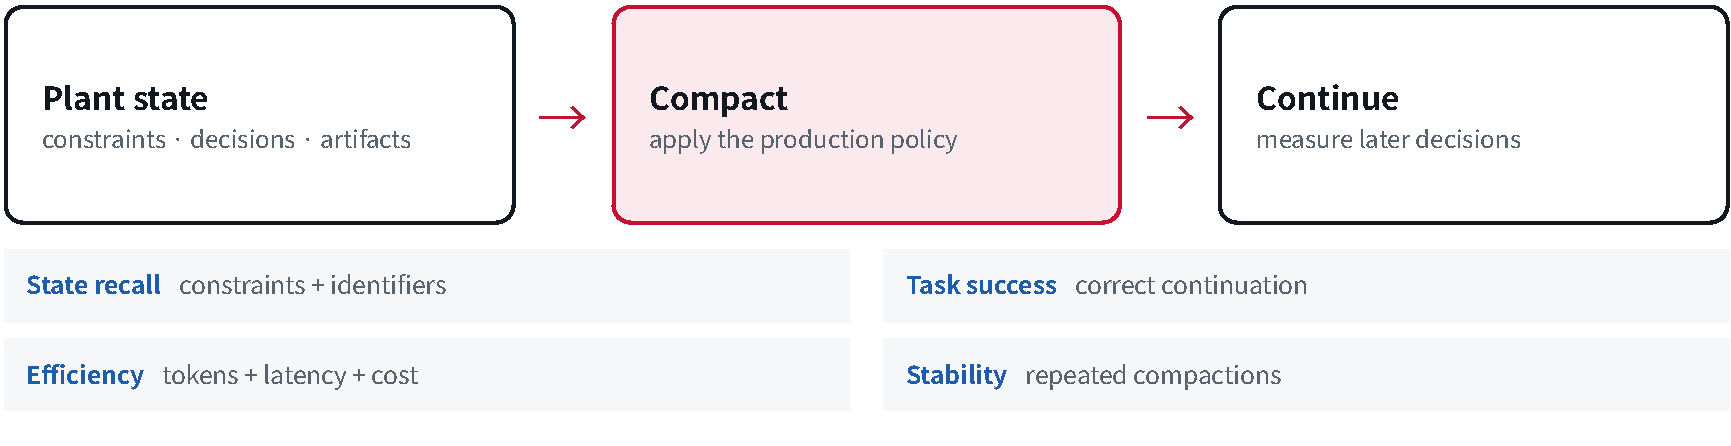
\includegraphics[width=\textwidth]{figures/基于继续任务的压缩评估.pdf}
\caption{官方课件第 51 页：先植入需要保留的状态，再应用生产压缩策略，最后观察继续任务的决策。\newline{\footnotesize 对应口述 01:12:01--01:14:03。}}
\end{figure}

有解释力的评测应覆盖四个维度：
\begin{itemize}
\item \textbf{状态保持}：精确约束、决定和对象标识符是否仍在后续行动中生效。
\item \textbf{任务成功}：Agent 是否继续正确方向、完成目标、避免重复外部动作。
\item \textbf{效率}：压缩调用本身、后续 token、时延和费用合计是否改善。
\item \textbf{稳定性}：多次压缩、用户中途修正、恢复旧证据时是否仍能保持行为。
\end{itemize}

\begin{importantbox}{评测摘要之后发生了什么}
要把约束、已完成动作和证据标识符放进历史，再让 Agent 真正继续执行。摘要读起来流畅，却丢失“这件事已经做过”或“这个版本号不可更改”，仍然可能让任务失败。
\end{importantbox}

\subsection{本章小结}

\begin{itemize}
\item Compaction 估计一个预算内的工作状态，目标是保持后续任务行为，而非单纯缩短文字。
\item 锚点、检查点、最近尾部与外部证据分别承担不同职责；用户中途的有效修正同样需要保留。
\item 触发预算、有效切分、替换格式和失败恢复共同构成完整策略。
\item 多次压缩会累积遗漏，评价需要覆盖继续任务、多轮交互和重复压缩。
\end{itemize}

\clearpage
\section{总结与延伸：长上下文是贯穿整个 Agent 系统的问题}

\subsection{讲者的收束：五个互相依赖的层次}

讲者最后把课程收束为五层：Agent 循环推动历史增长；推理阶段产生不同瓶颈；架构决定访问与保留历史的方式；缓存减少旧前缀重算；当预算仍然不足时，压缩要保留继续行动所需的状态。课件最后的完整总结如下。

\begin{figure}[H]
\centering
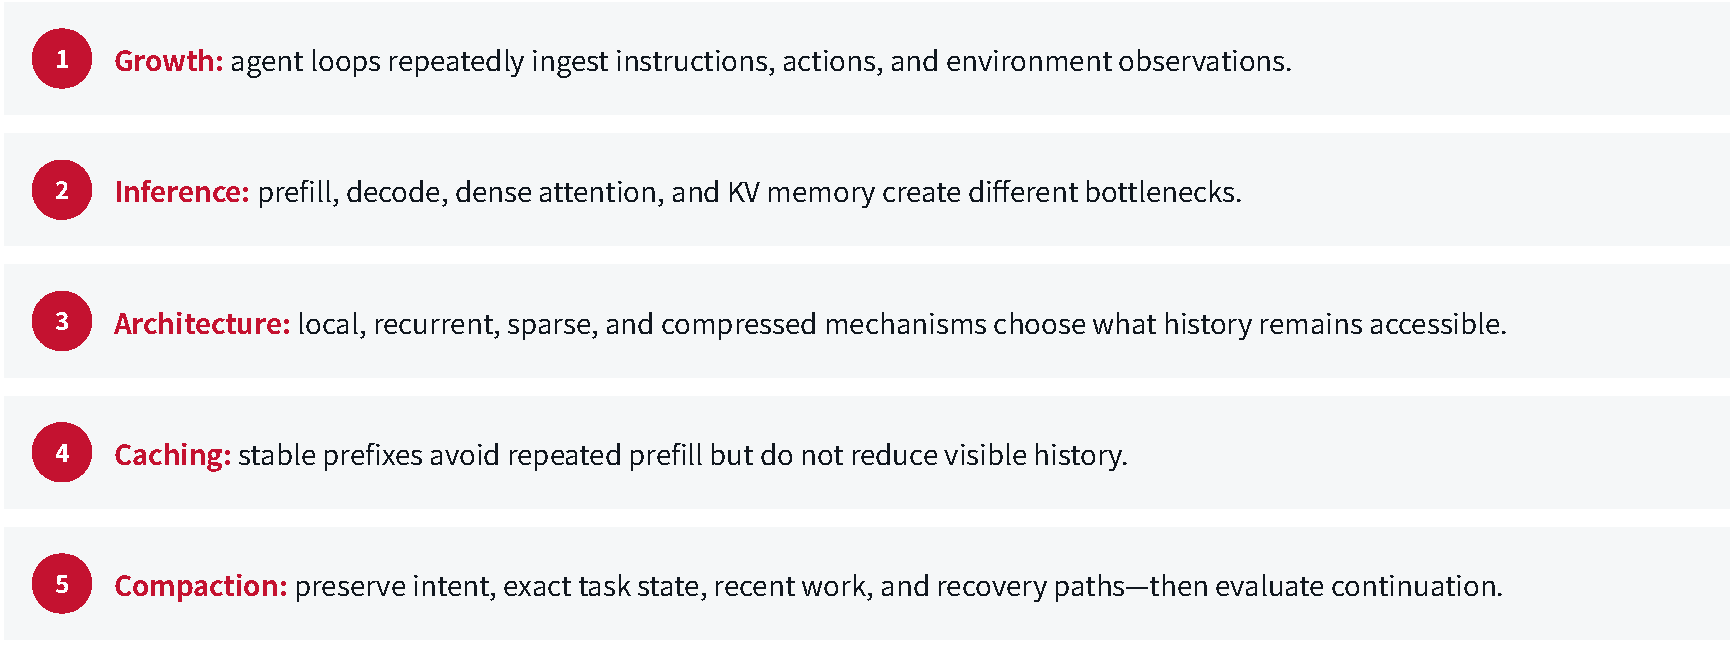
\includegraphics[width=\textwidth]{figures/长上下文系统五层总结.pdf}
\caption{官方课件第 53 页：从历史增长到行为保真的长上下文系统栈。\newline{\footnotesize 对应口述 01:14:03--01:14:52。}}
\end{figure}

\begin{enumerate}
\item \textbf{Growth}：每轮都带来指令、动作与环境观察，旧历史又会被再次纳入后续调用。
\item \textbf{Inference}：prefill、decode、稠密注意力和 KV 存储分别形成计算与内存压力。
\item \textbf{Architecture}：局部、递归、稀疏或压缩机制决定哪些信息仍可直接访问、哪些信息进入较短的状态。
\item \textbf{Caching}：稳定前缀可复用已有计算，但可见历史并未因此变短。
\item \textbf{Compaction}：保护意图、精确状态、近期工作和恢复路径，再通过继续任务验证质量。
\end{enumerate}

\subsection{课程归纳：容量、效率和行为应分别检查}

把这五层与长上下文训练连接起来，可以得到三个相互关联的检查问题。

\textbf{能装下多少？}位置编码和长度扩展、长序列训练、上下文并行、架构的状态表示，共同决定可处理的长度与资源需求。配置一个大窗口还不足以证明模型学会了利用远处信息；训练数据需要包含有意义的长距离依赖。

\textbf{重复读历史要付多少？}prefill 与 decode 的成本结构不同；KV 组织、精确前缀复用、路由和淘汰影响实际运行效率。缓存命中率高的会话仍可能占用大量 KV，长输出也仍有生成成本。

\textbf{继续做事是否可靠？}可访问的信息与模型真正能使用的信息可能有差距。改变架构或压缩历史后，要检查远距离证据、精确约束、中途修正和已完成动作是否还影响后续决策。

\begin{importantbox}{串起本课的主线}
先看 Agent 怎样增长历史，再识别 prefill、decode 与 KV 的具体瓶颈；用合适的架构和训练提高长序列处理能力，用缓存减少重复计算，最后用可恢复且经过继续任务评价的压缩状态控制工作历史。
\end{importantbox}

\subsection{课堂留下的边界与后续主题}

\begin{itemize}
\item \textbf{混合机制如何配合？}高效架构、上下文并行和服务内核需要兼容；理论上节约计算的机制，也要有能正确训练和执行的系统实现。
\item \textbf{缓存如何兼顾命中与容量？}更长保留时间提高潜在复用，却占用显存或其他存储；更积极的淘汰释放空间，也可能造成重算。
\item \textbf{压缩如何维持跨轮行为？}单次摘要质量不能回答多轮漂移、用户修正和外部动作去重问题，需要与任务继续结合评价。
\end{itemize}

最后的问答提到：子 Agent 也可以作为管理上下文的办法，把局部任务放入独立上下文，再带回有用结果。讲者确认这个方向有效，并将其留给后续课程讨论；本课没有展开调度、通信或隔离机制。下一讲进入 Skills and Memory，把关注点继续扩展到跨会话、较长时间范围内的能力与记忆。

\subsection{材料来源与进一步阅读}

\textbf{课程主材料}：Graham Neubig 的\href{https://www.youtube.com/watch?v=AiwCCvFW1uE}{L3 视频}、\href{https://www.cmu-agents.com/slides/lecture-03-long-context.pdf}{54 页官方课件}，以及\href{https://www.usetranscribe.io/yt/AiwCCvFW1uE/long-context-agents}{带时间公开转录}。正文图注中的页码指官方 PDF 页码；口述区间定位相应讲解。转录中的术语与数字结合课件核对。

前面各章已列出 Delta 规则、MLA、YaRN、Ring Attention、PagedAttention 与 SGLang 的原始阅读入口。以下补齐几条重要机制的来源：
\begin{itemize}
\item \href{https://arxiv.org/abs/2006.16236}{Transformers are RNNs}：线性注意力及递推状态表示。
\item \href{https://arxiv.org/abs/2412.06464}{Gated Delta Networks}：结合遗忘与 Delta 误差纠正。
\item \href{https://arxiv.org/abs/2510.26692}{Kimi Linear}：KDA 的逐通道遗忘与混合架构。
\item \href{https://arxiv.org/abs/2311.04934}{Prompt Cache}：可复用模块、位置管理与缓存读取实验。
\item \href{https://arxiv.org/abs/2606.13361}{Can I Buy Your KV Cache?}：课件第 39 页采用的缓存成本摊销研究。
\item \href{https://lmsys.org/blog/2024-12-04-sglang-v0-4/}{SGLang v0.4 的缓存感知路由}：把前缀复用与服务负载共同用于请求路由。
\end{itemize}

\subsection{本章小结}

长上下文需要模型、训练、推理服务和 Harness 一起工作。架构选择决定信息的表示与可访问性，缓存复用计算，压缩控制当前工作历史；最终评价都要回到 Agent 的后续动作和任务结果。

\end{document}
